%
\documentclass[apj]{emulateapj}
\bibliographystyle{apj}
%
\usepackage{apjfonts}
\usepackage{graphicx}
\usepackage{color}
\usepackage{amsbsy}
\usepackage{mathpazo,bm}
\usepackage{amsmath}
\usepackage{multirow}
\usepackage{natbib}
\usepackage{amssymb}
%
\newlength{\hfwidth}
\newlength{\hfwidthsingle}
\addtolength{\hfwidthsingle}{.5\textwidth} %single fig in figure
\addtolength{\hfwidth}{.497\textwidth} %single fig in figure*
%
\newcommand{\pderiv}[2]{\frac{\partial #1}{\partial #2}}
\newcommand{\pderivn}[3]{\frac{\partial^{#3} #1}{\partial #2^{#3}}}
\newcommand{\vt}[1]{\mathbf{#1}}       %for tensors
\renewcommand{\v}[1]{{\boldsymbol{#1}}} %for vectors
\def\white#1{\textcolor{white}{#1}}
\def\blue#1{\textcolor{blue}{ #1}}
\def\red#1{\textcolor{red}{#1}}
\definecolor{brown}{rgb}{0.42,0.24,0.07}
\def\brown#1{\textcolor{brown}{#1}}
\newcommand{\comm}[1]{({\it \brown{#1}})}
\newcommand{\del}{\v{\nabla}}
\newcommand{\grad}{\del}
\newcommand{\Div}{\del\cdot}
\newcommand{\Divp}[1]{\del\cdot\left(#1\right)}
\newcommand{\curl}{\del\times}
\newcommand{\Laplace}{\nabla^2}
%
\newcommand{\Eq}[1]{Eq. (\ref{#1})}
\newcommand{\Eqs}[2]{Eqs. (\ref{#1}) and~(\ref{#2})}
\newcommand{\Eqss}[2]{Eqs. (\ref{#1})--(\ref{#2})}
\newcommand{\eq}[1]{\Eq{#1}}
\newcommand{\eqs}[2]{\Eqs{#1}{#2}}
\newcommand{\eqss}[2]{\Eqss{#1}{#2}}
\newcommand{\eqp}[1]{(Eq. \ref{#1})}
%
\newcommand{\App}[1]{Appendix~\ref{#1}}
\newcommand{\app}[1]{\App{#1}}
\newcommand{\Figure}[1]{Figure~\ref{#1}}
\newcommand{\Fig}[1]{Fig.~\ref{#1}}
\newcommand{\fig}[1]{\Fig{#1}}
\newcommand{\Figs}[2]{Figs.~\ref{#1} and \ref{#2}}
\newcommand{\sect}[1]{Sect.~\ref{#1}}
\newcommand{\capsect}[1]{Section~\ref{#1}}
%
\newcommand{\beq}{\begin{equation}}
\newcommand{\eeq}{\end{equation}}
\newcommand{\beqn}{\begin{eqnarray}}
\newcommand{\eeqn}{\end{eqnarray}}
\newcommand{\epsp}{\xi_{_{+}}}
\newcommand{\epsm}{\xi_{_{-}}}
\newcommand{\tilchi}{\tilde\chi}
\newcommand{\tauf}{\tau_{\rm \blue{f}}}

\newcommand{\St}{{\rm St}}

\shorttitle{Dust in disk vortices}
\shortauthors{Lyra \& Lin}

\slugcomment{Draft version}

\begin{document}

\title{Steady state of dust distributions in disk vortices{\blue:}\\
\blue{Observational predictions and applications to transitional disks}}
\author{Wladimir Lyra\altaffilmark{1,2,3,$\star$} and Min-Kai Lin\altaffilmark{4,$\star$}}
\email{wlyra@caltech.edu, \ mklin924@cita.utoronto.ca}
\altaffiltext{1}{Jet Propulsion Laboratory, California Institute of Technology, 4800 Oak Grove Drive, Pasadena, CA, 91109, USA}
\altaffiltext{2}{Division of Geological \& Planetary Sciences, California Institute of Technology, 1200 E California Blvd MC 150-21, Pasadena, CA 91125 USA}
\altaffiltext{3}{Sagan Fellow}
\altaffiltext{4}{Canadian Institute for Theoretical Astrophysics , 60
  St. George Street, Toronto, Ontario, M5S 3H8, Canada}
\altaffiltext{$\star$}{Both authors contributed equally to this work}

\begin{abstract}
The Atacama Large Millimeter Array (ALMA) has been  returning images of transitional disks in which large asymmetries are seen in the dust distribution of 
mm-size in the outer disk. The explanation in vogue borrows from the vortex literature by suggesting 
that these asymmetries are the result of dust trapping in giant vortices, excited via Rossby wave instability (RWI) 
at planetary gap edges. Due to the drag force, dust trapped in vortices will accumulate 
in the center\blue{, and} diffusion is needed to maintain a steady state over the lifetime of the disk. While previous work 
derived semi-analytical models of the process, in this paper we
provide analytical steady-steady solutions. \blue{Exact solutions exist for certain vortex models.}
The solution is determined by the vortex rotation profile, the gas scale height, the 
vortex aspect ratio, and the ratio of dust diffusion to gas-dust friction. In principle, all these quantities can be derived
from observations, which would give validation of the model, also giving constrains on the strength of the turbulence 
inside the vortex core.  \blue{Based on our solution, we derive quantities such as the gas-dust contrast, the trapped dust mass,
and the dust contrast at the same orbital location. We apply our model to the recently imaged Oph IRS 48 system, finding 
values within the range of the observational uncertainties.}
\end{abstract}

\section{Introduction}
\label{sect:introduction}

Transitional disks are a class of circumstellar disks that lack a
significant near-infrared (1-5$\mu$m) excess, while showing steep
slopes in mid-infrared (5-20$\mu$m) and
far-infrared ($>$20$\mu$m) excesses typical of classical T-Tauri disks
\citep{Strom89,Skrutskie90,Gauvin-Strom92,Wolk-Walter96,Calvet02,Calvet05,Muzerolle06,Sicilia06,Currie09,Currie-Sicilia11}. 
This ``opacity hole''  implies absence of optically thick warm dust in the inner disk, with a dust
wall generating the mid-IR emission, followed by cold dust in the
outer disk.  This, together with their age (in the 1-10 Myr range, see
e.g. \citealt{Currie10} for a review) provide strong evidence that these are
objects caught in the evolutionary stage between gas-rich 
primordial and gas-poor debris disks, hence the name. 

Explanations for the opacity hole generally fall in four distinct
categories. These are, namely, grain growth and dust settling \citep{Brauer07,Dominik-Dullemond08,Zsom11,Birnstiel12}, photoevaporation
\citep{Alexander06,Cieza08,Pascucci-Sterzik09,Owen10}, 
dynamical interaction with close stellar or substellar companions
\citep{Ireland-Kraus08}, and planet
formation via dust locking \citep{Safronov69,Lyttleton72,Goldreich-Ward73,Youdin-Shu02,Johansen07} and gap
carving \citep{Papaloizou-Lin84,Lin-Papaloizou86a,Lin-Papaloizou86b,Bryden99,Paardekooper-Mellema04,Quillen04,Najita07,Andrews11}. 
Analyses of individual disks \citep{Calvet04,Calvet05,Espaillat08} tend to favor one process over another, and even census
studies of statistically significant samples of disks find one process
to be dominant \citep{Najita07,Cieza08}. These
seemingly conflicting results in fact illustrate the
heterogeneity of transitional disks, where a combination of all
suggested processes are needed to explain the rich diversity observed 
\citep{Cieza10,Muzerolle10,Merin10,Rosotti13,Clarke-Owen13}.   

Recently, high angular resolution imaging of the outer regions of transitional 
disks have become available, showing a myriad of puzzling asymmetries 
that beg for explanation. These come in the shape of spiral arms
\citep{Pietu05,Corder05,Muto12,Tang12},  elliptical dust walls
\citep{Isella12}, and non-axisymmetric dust clouds
\citep{Oppenheimer08,Brown09,Casassus12}. In particular, giant horseshoe-shaped dust distributions are seen in images obtained with \blue{the Combined Array for Research in Millimeter-wave Astronomy 
(CARMA, \citealt{Isella13})} and with the \blue{Atacama Large Millimeter Array} (ALMA, \citealt{Casassus13,vanderMarel13}). The planet interpretation is particularly attractive for 
explaining these asymmetries, since they generally match the range of structures predicted by hydrodynamical 
models of planet-disk interaction. 

A deep gap is one of these expected structures, as the planet tides expel material from the vicinity of its orbit 
\citep{Papaloizou-Lin84,Lin-Papaloizou86a,Lin-Papaloizou86b,Nelson00,Masset-Snellgrove01,Paardekooper-Mellema04,Quillen04,deValBorro06,Klahr-Kley06,Lyra09a,Zhu11,Kley12}. 
The gas gap has sharp walls, that constitute a steep pressure gradient, modifying the rotational profile locally. 
This situation is prone to excite what has been called Rossby wave
instability (RWI), that are in fact  ``edge modes'' 
\citep{Lovelace-Hohlfeld78,Toomre81,Papaloizou-Pringle84,Papaloizou-Pringle85,Hawley87,Lovelace99,Varniere-Tagger06,deValBorro07,Lyra08,Lyra09a,Lyra09b,
Meheut10,Meheut12a,Meheut12b,Meheut12c,Lin-Papaloizou11a,Lin-Papaloizou11b,Lin-Papaloizou12,Lyra-MacLow12,Lin12,Lin13} 
akin to Kelvin-Helmholtz instability, thus converting the extra shear
into vorticity. The large-scale vortices that result are well-known to trap 
dust, a property that has been invoked in the context of primordial disks to
speed up planet formation by trapping solids of cm to m size \citep{Barge-Sommeria95,Adams-Watkins95,Tanga96,Klahr-Henning97,Hodgson-Brandenburg98,Chavanis00,delaFuenteMarcos-Barge01,Johansen04,Inaba-Barge06}, and demonstrated through numerical simulations to efficiently achieve the
critical densities needed for gravitational collapse \blue{of the
  trapped clumps} \citep{Lyra08,Lyra09a,Lyra09b}. 

Part of these results have been applied to the field of
transitional disks. The particle size that is
preferentially trapped is set by the friction time, $\tauf$, which is a
function of the gas density and particle radius. A suitable nondimensionalization for the
friction time is the Stokes number, $\St = \varOmega \tauf$,
where $\varOmega$ is the Keplerian frequency. Dust that is too
well-coupled to the gas ($\St\rightarrow 0$) does not suffer friction, and bodies
that are too large ($\St\rightarrow \infty$) have too much inertia to be moved by the
gas: the preferential size for trapping is \St=1 (see e.g. \citealt{Youdin-Goodman05,Youdin08}).
While in the dense, fast rotating, inner regions of primordial disks, 
the preferentially trapped particle size corresponds to meter-size, in
the thin, slowly rotating, outer regions of transitional
disks, the size corresponding to \St=1 drops by about three orders of
magnitude \blue{\citep{Brauer07,Pinilla12a}}. The resulting trapping of sub-mm and mm-size dust may not
lead to the critical densities necessary to form planets, but they may
well explain the puzzling observed lopsided asymmetries. While the 
motivation and particle sizes are different, the relevant physics 
is scale-free, and thus identical as long as gravity is not involved. 

This property was invoked by \citet{Regaly12} to suggest that the 
sub-mm observations of \citet{Brown09} could be the result of dust
trapping in Rossby vortices. If indeed that is the case, then, 
as the drag force drives dust toward the vortex center, diffusion is
needed to maintain a steady state over the lifetime of the disk
\citep{Klahr-Henning97,Chavanis00}. \citet{Birnstiel13} presented a semi-analytical model that solves for the azimuthal dust 
distribution while using fits from numerical simulations
\citep{Pinilla12b} to constrain the radial morphology. In this work we present an analytical 
model for the steady state distribution of dust trapped in vortices, 
accurate to first order in Stokes number, and general in space. In 
\sect{sect:model-equations} we derive the
advective-diffusive equation, and in \sect{sect:coordinate-transformation} the appropriate coordinate
transformation. In \sect{sect:axisymmetric} we solve the equation for
the ``axisymmetric'' case \blue{in that coordinate system}, and in
\sect{sect:nonaxisymmetric}  we generalize it for
non-axisymmetry. \blue{In \sect{sect:observables} 
we derive observational predictions, and apply the model to the Oph IRS 48 system.}

\section{Dust steady state} 
\label{sect:model-equations}

Considering the dust is of small sizes, we can treat it as a
fluid. The dust should then follow the continuity equation 

\beq
  \pderiv{\rho_d}{t} = -(\v{\blue{w}}\cdot\del)\rho_d - \rho_d \Div{\v{\blue{w}}} - \blue{\Div{J}}
%\blue{\Div{\left(D\,\rho_g\grad\varepsilon\right)}},
  \label{eq:continuity-w}
\eeq

\noindent where $\rho_d$ is the dust density, $\v{w}$ is the dust
velocity, \blue{and $J$ is the diffusion flux. We take it to be}
 
\beq 
\blue{J=-D\,\rho_g\grad{\left(\rho_d/\rho_g\right)}}\label{eq:j-flux}
\eeq 

\noindent \blue{as in the contaminant equation
\citep{Morfill-Volk84,Clarke-Pringle88,Charnoz11},} where $D$ is the  
diffusion coefficient (the diffusion is due
to elliptical turbulence in the vortex core and in general will be
different than the turbulent viscosity in the disk), \blue{and $\rho_g$ is
the gas density}. We assume \blue{that} $D$ is constant. A list of the mathematical symbols used in this work, together
with their definitions, is provided in Table~\ref{table:symbols}. 

To derive the velocities, instead of solving the momentum equations
for the dust, we make use of the relative velocity, following
\citet[see also \citealt{Youdin08}]{Youdin-Goodman05}

\beq
\blue{\v{w}} = \v{u} + \tauf  \grad{h}, 
\label{eq:w}
\eeq
\noindent where $\v{u}$ is the gas velocity. \eq{eq:w} is 
accurate to first order in friction time $\tauf$, assumed 
constant. \blue{For isentropic gas, t}he enthalpy $h$ is defined as $dh = dp /\rho_g$, where $p$ 
is the pressure. \blue{As noted by
\cite{Charnoz11}, \eq{eq:continuity-w} can be written as a typical continuity equation with Laplacian diffusion 
\beq
\partial_t \rho_d = -(\v{v} \cdot\del)\rho_d - \rho_d \Div{\v{v}} + D\Laplace\rho_d \label{eq:continuity}
\eeq
\noindent provided that the effective velocity $\v{v}$ is 
\beq
\v{v} \equiv \v{w}  + D\grad\ln \rho_g\label{eq:v-prime}.
\eeq\noindent For isothermal gas the extra term is $D/c_s^2 \grad{h}$,
and, comparing with \eq{eq:w}, its effect amounts to redefining the
friction time as 
\beq
\tau \equiv \tauf + \frac{D}{c_s^2}\label{eq:tau-prime}
\eeq
\noindent combining \eq{eq:w}, \eq{eq:v-prime} and \eq{eq:tau-prime},
we can thus write
\beq
\blue{\v{v}} = \v{u} + \tau \grad{h}, \label{eq:v}
\eeq \noindent valid for isothermal gas only.}

Inside the vortex, the gas flow is divergenceless, and 
we adopt the following model for $\v{u}$
\beq
  u_x = \varOmega_V y / \chi \qquad  u_y= -\varOmega_V x \chi,
  \label{eq:vortex}
\eeq
\noindent where $\chi > 1$ is the vortex aspect ratio (it has
semi-minor axis $a$ and semimajor axis $a\chi$). \blue{Notice that the flow eventually
  gets supersonic for large values of $x$ and $y$. This will limit the
  validity of the solution, as the vortices shock beyond the sonic
  perimeter. This effectively leads to a vortex ``boundary'', beyond
  which the motion resumes to the background Keplerian flow.} 

In this work we consider the Kida solution \citep{Kida81}

\beq
\varOmega_V = \frac{3\varOmega}{2(\chi-1)},  
\eeq
which smoothly matches the above velocity field to the Keplerian
shear; as well as the GNG solution \citep{Goodman87}, that exactly solves the 
compressible Euler equations 

\beq
\varOmega_V=\varOmega\sqrt{3/(\chi^2-1)}.
\eeq

\blue{We comment that these solutions make use of the shearing box
  equations, and are thus subject to the same limitations as that
  approximation \citep{Regev-Umurhan08}. In
  particular, the shearing box does not have a radial vorticity
  gradient, and thus cannot excite the RWI
  \citep{Tagger01}. Nevertheless, independently of the excitation
  mechanism, these solutions are good local descriptions of the perturbed
  flow. The GNG solution was used to model vortices
  found in non-linear hydrodynamic global simulations of the
  Papaloizou-Pringle instability \citep{Hawley87}, which is similar to
  the RWI. Recently, \cite{Lin-Papaloizou11a} found that, in
  quasi-steady state, the RWI vortices excited at planetary gap edges 
  resemble vortices formed by perturbing the disk with
  the Kida solution. We are thus confident that the above solutions are suitable
  as a first model for disk vortices.  Moreover, it is straight forward
  to generalize the solutions below to any flow in the form
  $u_x\propto y$ and $u_y\propto -x$.}

We note that the dust velocity \blue{\eqp{eq:v}} is comprised of a divergent-free part, $\v{u}$, and a
curl-free part, $\tau\grad{h}$. The vortex flow attempts to keep the
dust particles on closed elliptic streamlines via $\v{u}$, while friction
attempts to concentrate dust toward pressure maximum via $\tau\grad{h}$. The only effect that attempts to spread out the dust is diffusion
via $D$.  

Taking the divergence of
\eq{eq:v} gives 

\beq
\Div{\v{v}} = \tau \Laplace{h}, 
\label{eq:divv}
\eeq

\noindent and we can find the Laplacian of the enthalpy via the Euler
equation. Adopting the shearing sheet approximation, in steady state
the force balance yields  

\begin{eqnarray}
\pderiv{h}{x} &=& 3\varOmega^2 x + 2\varOmega u_y -
u_y\pderiv{u_x}{y} \nonumber \\
&=& \left(3\varOmega^2 - 2\varOmega\varOmega_V \chi + \varOmega_V^2\right) x
= -\frac{C_1}{\tau} \  x,  \label{eq:gas_mom1}\\
\pderiv{h}{y} &=& - 2\varOmega u_x -
u_x\pderiv{u_y}{x} \nonumber \\
&=& \left(-2\varOmega\varOmega_V/\chi + \varOmega_V^2\right) y = -\frac{C_2}{\tau} \  y.\label{eq:gas_mom2}
\end{eqnarray}

\noindent  Substituting the equations above into \eq{eq:divv}, also
with $\omega_{_V}=\varOmega_V/\varOmega$, the divergence becomes 

\beqn
\Div{\v{v}} &=& -(C_1+C_2) = - C \label{eq:const-div}\\
&=& - \tau\varOmega^2
\left[2\omega_{_V}\left(\frac{\chi^2+1}{\chi}\right) - (2\omega_{_V}^2
  + 3) \right], 
\label{eq:scale-div}
\eeqn

\noindent where we define $C$ as positive, so that the divergence is
negative (physically meaning that the dust gets trapped). Replacing
\eq{eq:const-div} in the \blue{modified} continuity equation \blue{\eqp{eq:continuity}}, and setting $\partial_t$ =
0 for steady state, 

\beq
\left(D\Laplace{} -  \v{v}\cdot\del  + C\right)\rho_d = 0. 
\label{eq:steady}
\eeq

Substituting the gas velocity \blue{\eqp{eq:vortex}}, and dividing by $D$, we
arrive at the modified advection-diffusion equation that should
determine the steady-state distribution of the vortex-trapped dust, 

\beq
\left[\Laplace{} - \left(Ay\chi^{-1} - B_1x\right) \partial_x  +
  \left(A x \chi + B_2y\right) \partial_y + B \right] \rho_d   = 0,  
\label{eq:dust-trapping-cartesian}
\eeq
\\
\noindent where we also substituted  $A=\varOmega_V/D$ and $B_i=C_i/D$.

\begin{table}
\caption[]{Symbols used in this work}
\label{table:symbols}
\begin{center}
\begin{tabular}{l l l}\hline
Symbol & Definition & Description \\\hline
$\tauf$ && friction time\\
$D$ & & dust diffusion coefficient \\
$c_s$ & & sound speed \\
$\blue{\tau}$ &\blue{=$\tauf + D/c_s^2$}& \blue{effective friction time}\\
$\varOmega$ & & Keplerian angular frequency \\
\St & $= \varOmega \tauf$ & Stokes number \\
$t$ &  & time \\
$\rho_g$, $\rho_d$  & & gas and dust density\\
$\v{u}$, \blue{$\v{w}$} & & gas and dust velocity\\
\blue{$\v{v}$} & \blue{$= \v{w} + D\grad\ln\rho$}& \blue{effective dust velocity} \\
$p$ && gas pressure \\
$h$ &$dh=dp/\rho_g$ & gas enthalpy\\
$\chi$ & & vortex aspect ratio ($>1$) \\
$a$ & & vortex semi-minor axis \\
$\varOmega_V$ & & vortex angular frequency \\
$\omega_{_V}$ &  $=\varOmega_V$/$\varOmega$ & dimensionless vortex frequency  \\
$C$ & $=-\Div{\v{v}}$ &  \\
$A$ & $=\varOmega_V/D$ & \\
$B$  &$=C/D$ & \\
$\nu$ & & azimuth in vortex reference frame\\
$\xi_\pm$ & $ = 1\pm\chi^{-2}$ \\
$H$ & $c_s/\varOmega$ & sonic scale, gas scale height\\
$\delta$ & $D=\delta c_s H$ & dimensionless diffusion parameter\\
$f(\chi)$ & \eq{eq:scale-function} & scale function \\
\blue{$S$} & \blue{$= \St/\delta$} & \blue{dimensionless number} \\
\blue{$H_g$} & \blue{$=H/f(\chi)$} & \blue{gas vortex scale length} \\
$H_V$ & $=H_g \sqrt{\blue{\frac{1}{S+1}}}$ & \blue{dusty} vortex scale length \\
$k$ & $=\sqrt{2}/H_V$ & \\ 
$\blue{\zeta}$ & $=ka$ & \\
$\tilchi$ & $=\frac{\chi^2-1}{2(\chi^2+1)}$ & \\
\blue{$\beta$} & \blue{$=(B_1-B_2)/4B$}& \\
$k_m$ & $= 1+imA/B$ & \\
$\mathcal{A}_m$ $\mathcal{B}_m$ $\mathcal{C}_m$  &\eqss{eq:ops}{eq:opsw} & differential operators \\
\blue{$b_m$} & & constants\\
$\epsilon(\blue{\zeta})$ & & non-axisymmetric correction \\
\blue{$\varepsilon$} & \blue{$=\int \rho_d dV/ \int \rho_g dV$}& \blue{global dust-to-gas ratio}\\
\blue{$\rho_0$} & & \blue{max gas density, reference density} \\
 & & \\ \hline
\end{tabular}
\end{center}
\end{table}


\section{Change of variable}
\label{sect:coordinate-transformation}

We change variables to the coordinate system used in \citet{Chang-Oishi10}

\beqn
  x &=& a \cos\nu, \label{eq:change-x}\\
  y &=& a\chi\sin\nu.  \label{eq:change-y}
\eeqn

The system is not orthogonal, but it has the advantage of matching the
aspect ratio of the ellipses. (In contrast, the elliptic coordinate
system, though orthogonal, describes a system of confocal ellipses of
different aspect ratio, that does not coincide with the geometry of
the problem.) In these coordinates, the transformations are 

\beq
\left[\begin{array}{c}
    \partial_{a}  \\
    \partial_{\nu}
  \end{array}\right] = \vt{A} 
  \left[\begin{array}{c}
      \partial_{x}  \\
      \partial_{y}
    \end{array}\right] 
%
\quad {\rm and} \quad 
%
\left[\begin{array}{c}
    \partial_{x}  \\
    \partial_{y}
  \end{array}\right] = \vt{A}^{-1} 
  \left[\begin{array}{c}
      \partial_{a}  \\
      \partial_{\nu}
    \end{array}\right],  
%
\eeq

\noindent with 

\beq
\vt{A} = \left[\begin{array}{cc}
\pderiv{x}{a}  & \pderiv{y}{a}  \\
\pderiv{x}{\nu}  & \pderiv{y}{\nu} \\
\end{array}\right] = \left[\begin{array}{cc}
\cos\nu  & \chi\sin\nu  \\
-a\sin\nu  & a\chi\cos\nu \\
\end{array}\right]. 
\eeq

\noindent The inverse matrix is 

\beq
\vt{A}^{-1} = \frac{1}{a\chi} \left[\begin{array}{cc}
a\chi\cos\nu  & -\chi\sin\nu  \\
a\sin\nu  & \cos\nu \\
\end{array}\right].  
\eeq

The transformations are therefore

\beqn
\pderiv{}{x} &=& \cos\nu \pderiv{}{a} - \frac{\sin\nu}{a} \pderiv{}{\nu}, \\
\pderiv{}{y} &=& \frac{1}{\chi}\left(\sin\nu \pderiv{}{a} + \frac{\cos\nu}{a} \pderiv{}{\nu} \right),
\eeqn

\noindent and the Laplacian is thus 

\beqn
\Laplace{} &= &\frac{1}{2}\left[ \epsm \cos 2\nu +  \epsp\right] \partial^2_a  \nonumber \\
                &+& \frac{1}{2a^2}\left[ \epsp - \epsm \cos 2\nu\right] \partial^2_\nu \nonumber \\
                &-& \frac{\sin 2\nu}{a}\epsm \partial^2_{a\nu}   \nonumber \\
                &+& \frac{1}{2a}\left[ \epsp - \epsm \cos 2\nu\right] \partial_a \nonumber \\
                &+& \frac{\sin 2\nu}{a^2} \epsm\partial_\nu, \label{eq:laplace}
\eeqn

\noindent with $\xi_{\pm} = (1 \pm \chi^{-2})$.  As for the advection term, we have 

\beqn
\v{v}\cdot\del &=& (\v{u} + \tau \grad h) \cdot \del \nonumber \\
&=& - \left[\varOmega_V - \frac{\sin2\nu}{2}  (C_1 -  C_2)\right]\partial_\nu \nonumber \\
&&- \left( C_1 \cos^2\nu   + C_2\sin^2\nu \right) a \ \partial_a. \label{eq:advection-term}
\eeqn

The dust-trapping equation is therefore 

\beqn 
&& \left\{ \Laplace{} + \left[A - \frac{\sin2\nu}{2}  (B_1 - B_2)\right]\partial_\nu \ +  \right.  \nonumber\\
&& \left. \white{\frac{1}{1}}\left( B_1 \cos^2\nu   + B_2\sin^2\nu
  \right) a \ \partial_a  + B \right\} \rho_d = 0. \label{eq:dust-trapping-uvzero}
\eeqn

%\blue{We remark that a very similar equation  can be derived  when the diffusive flux is modeled as $D\rho_g\nabla(\rho_d/\rho_g)$, as used by \cite{Birnstiel13} . In fact, by redefining the friction time, 
%our solution below can be made applicable to this case as well.} 

\section{``Axisymmetric'' \blue{solution}}
\label{sect:axisymmetric}

\blue{\subsection{Dust distribution}}

We now make the assumption that the dust distribution follows, in shape, that of
the gas (we will relax this approximation in the next section). In this case, the
dust distribution follows ellipses of equal aspect ratio. So,
$\partial_\nu$ = 0, ``axisymmetric'' in the ($a,\nu$)
coordinates. \eq{eq:dust-trapping-uvzero} becomes

\beqn
&&\left\{\frac{1}{2}\left(\epsm \cos 2\nu +\epsp\right) \partial^2_a  +  \left[\frac{1}{2a}\left( \epsp - \epsm\cos 2\nu\right) \right.\right. \nonumber\\
&&\left.\left.\white{\frac{1}{1}}+ (B_1\cos^2\nu +  B_2\sin^2\nu)a\right] \partial_a  + B\right\} \rho_d = 0. \label{eq:axi}
\eeqn

We now integrate the above equation in $\nu$, from 0 to 2$\pi$. This yields

\beq\label{eq:dust-trapping-axis}
\left[\partial^2_a  +  \left(\frac{1}{a} +  \frac{k^2}{2}a\right) \partial_a  + k^2\right]\rho_d = 0, 
\eeq

\noindent where we define $k^2=2B/\epsp$. Note that the parameter $A$
is absent because it represents advection by the vortex, which only
move dust particles along the same ellipse, not across it. It is
not relevant in the $\nu$-averaged problem. The solution of
\eq{eq:dust-trapping-axis} is 

\beq
\rho_d(a) = \exp\left(-\frac{k^2a^2}{4}\right)  \left[c_1 + c_2 {\rm
    Ei}\left(\frac{k^2a^2}{4}\right)\right],
\eeq

\noindent where $c_1$ and $c_2$ are constants, and ${\rm Ei}(x)$ is
the exponential integral function. Since it diverges at the origin, $c_2$ has to be zero, and 

\beq
\rho_d(a) = \rho_{d\,{\rm max}} \ \exp\left(-\frac{a^2}{2H_V^2}\right),
\label{eq:gen_axi}
\eeq

\noindent with $H_V = \sqrt{2}/k$ for symmetry with the gas sonic scale. We can 
rewrite this length scale recalling that $k^2=2B/\epsp$ and
$B=C/D$. We can substitute the diffusion coefficient $D=\delta \varOmega H^2$ where 
$\delta$ is a dimensionless coefficient, and $\St = \tauf\varOmega$ for 
the Stokes number, writing thus 

\beqn
\label{eq:k}
k^2 = \frac{2\blue{(}\St+\blue{\delta)}}{\delta H^2} f^2(\chi),
\eeqn 

\noindent so

\beq
 H_V = \frac{H}{f(\chi)} \sqrt{\frac{\delta}{\St\blue{+\delta}}}. 
\label{eq:hv-pre}
\eeq
\noindent \blue{following \cite{Jacquet12} we define $S=\St/\delta$. The vortex scale
length is therefore
\beq
H_V = \frac{H}{f(\chi)} \sqrt{\frac{1}{S+1}}
\label{eq:hv}
\eeq}

\noindent In these equations, the scale function $f(\chi)$ is given by 

\beqn
f^2(\chi) &=& \epsp^{-1} \left[2\omega_{_V}\left(\frac{\chi^2+1}{\chi}\right) - (2\omega_{_V}^2 + 3) \right]\nonumber \\
          &=& 2\omega_{_V}\chi - \epsp^{-1}(2\omega_{_V}^2 + 3),
\label{eq:scale-function}
\eeqn

\noindent and depends on the vortex solution
used. We plot $f(\chi)$ for the Kida and GNG solutions in
\fig{fig:scale-function}. They are defined in the real axis only for $\chi > 2$ ($f^2
< 0$ for $0 < \chi < 2$ ). The Goodman solution tends to an asymptote
around 0.7. The Kida solution has a  tail around $0.5\pm0.25$ in the
interval of physical relevance ($2 < \chi \lesssim 10$). %The dust distribution is thus 

\begin{figure}
  \begin{center}
    \resizebox{\columnwidth}{!}{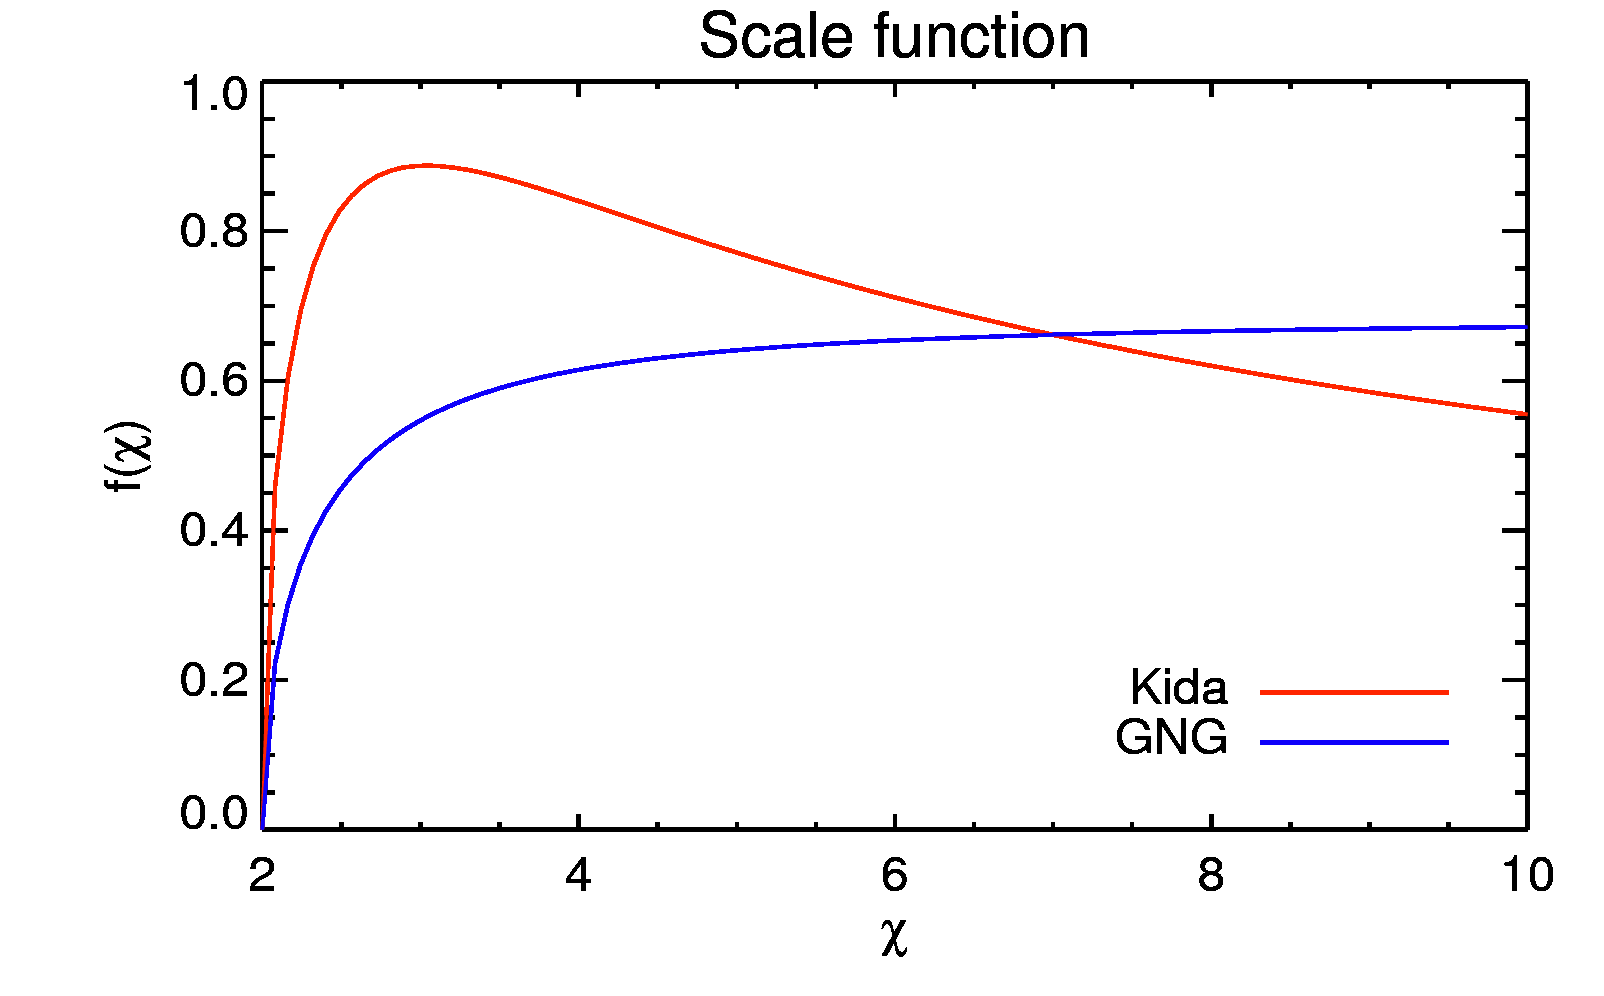
\includegraphics{../figs/scale_function.png}}
  \end{center}
\caption[]{The scale function $f(\chi)$, defined by
  \eq{eq:scale-function}, for the Kida ($\varOmega_V=3/2
  \ \varOmega_K/(\chi-1)$) and GNG ($\varOmega_V=\varOmega_K
  \sqrt{3/(\chi^2-1)}$) solutions, respectively. The scale function is
  related to the square root of the negative of the divergence
  \eqp{eq:scale-div}, and defined only for $\chi>2$. For smaller $\chi$ the
  divergence flips positive, meaning that dust is expelled from the
  vortex instead of getting trapped. This happens because of the
  correlation between $\varOmega_V$ and $\chi$. The aspect ratio shrinks
  as the vortex intensifies. At some point, the vortex rotates too
  fast, and particles are expelled by the centrifugal force.}
 \label{fig:scale-function}
\end{figure}

%Dust distributions for different values of \blue{$S$} are plotted in \fig{fig:gaussian}, as a 
%function of $a/H$. 
We show in \fig{fig:disk}, in the inertial frame, 
the dust distribution for \blue{$S$}=1 in a Kida vortex of $\chi=4$ embedded in a 
disk of aspect ratio $H/r$=0.1, where $r$ is the stellocentric
distance. \blue{We caution that this image extrapolates the spatial
range of applicability of the shearing box approximation used to construct
the solution.}

\blue{It is worth noting that for certain vortex models and/or
aspect-ratios, the Gaussian solution, \eq{eq:gen_axi}, is in fact an 
exact solution to the dust-steady state equation, \eq{eq:dust-trapping-uvzero}.  
We will explore this in more detail  in \sect{sect:nonaxisymmetric}, but one can check this by inserting
\eq{eq:gen_axi} into \eq{eq:dust-trapping-uvzero}, and finding the condition 
for the coefficient of the trigonometric terms to vanish. 
In this special case, explicitly averaging over $\nu$ is not
required to remove the $\nu$-dependence from the 
problem.} 

%\blue{For completeness, we present also the vertical dependency of the
%  dust distribution. It is straighforward and has already been
%  calculated by, e.g., \citet{Dubrulle95}). We take
%  the right-hand-side of the modified diffusion equation \eqp{eq:continuity}
%  \beq
%  -v_z\partial_z \rho_d - \rho_d\partial_z v_z + D\partial^2_z \rho_d  = 0 
%\eeq and substitute the terminal dust velocity $v_z = \tau \partial_z h =
%-\tau\varOmega^2 z$ (this step used the gas stratification $\ln \rho_g (z) =
%-z^2/2H^2$). Using the ansatz $\ln \rho_d (z) =-z^2/2H_d^2$, the equation
%above becomes 
%   \beq
%\left[\frac{D}{H_d^2} - \tau\varOmega^2\right] \left(\frac{z^2}{H_d^2} - 1\right) = 0 
%\eeq which is only true for all values of $z$ if $H_d^2 = D/(\tau\varOmega^2)$, i.e., 
%\beq
%H_d = H/\sqrt{{S+1}}
%\eeq
%} 

\blue{\subsection{Gas distribution}}

\blue{\eq{eq:gen_axi} allows us to calculate the gas distribution. For
  that we recall that  for tracer particles ($\St=0$), the dust distribution should
  mimic that of the gas. The distribution should thus be 
\beq
\rho_g(a) = \rho_{g\,{\rm max}} \ \exp\left(-\frac{a^2}{2H_g^2}\right), \label{eq:gas_axi}
\eeq
\noindent with 
\beq
H_g = {H_V}{\vert_{\St=0}} = H/f(\chi) \label{eq:hg}
\eeq \noindent and
$\rho_{g\,{\rm max}}$, the maximum gas density{\footnote{\blue{Note that 
\eq{eq:gas_axi} is the gas density averaged over $\nu$ at fixed $a$.  One may  
directly integrate the gas momenta equations to see that the gas
density/pressure depends, in general, on both $a$ and $\nu$.}}}. }

\blue{Notice that for $\St=0$ the effect of diffusion cancels out. This is because
the diffusion is proportional to the gradient of the dust-to-gas
ratio \eqp{eq:j-flux}, which is zero for tracer
particles.}



\begin{figure}
\begin{center}
  \resizebox{\columnwidth}{!}{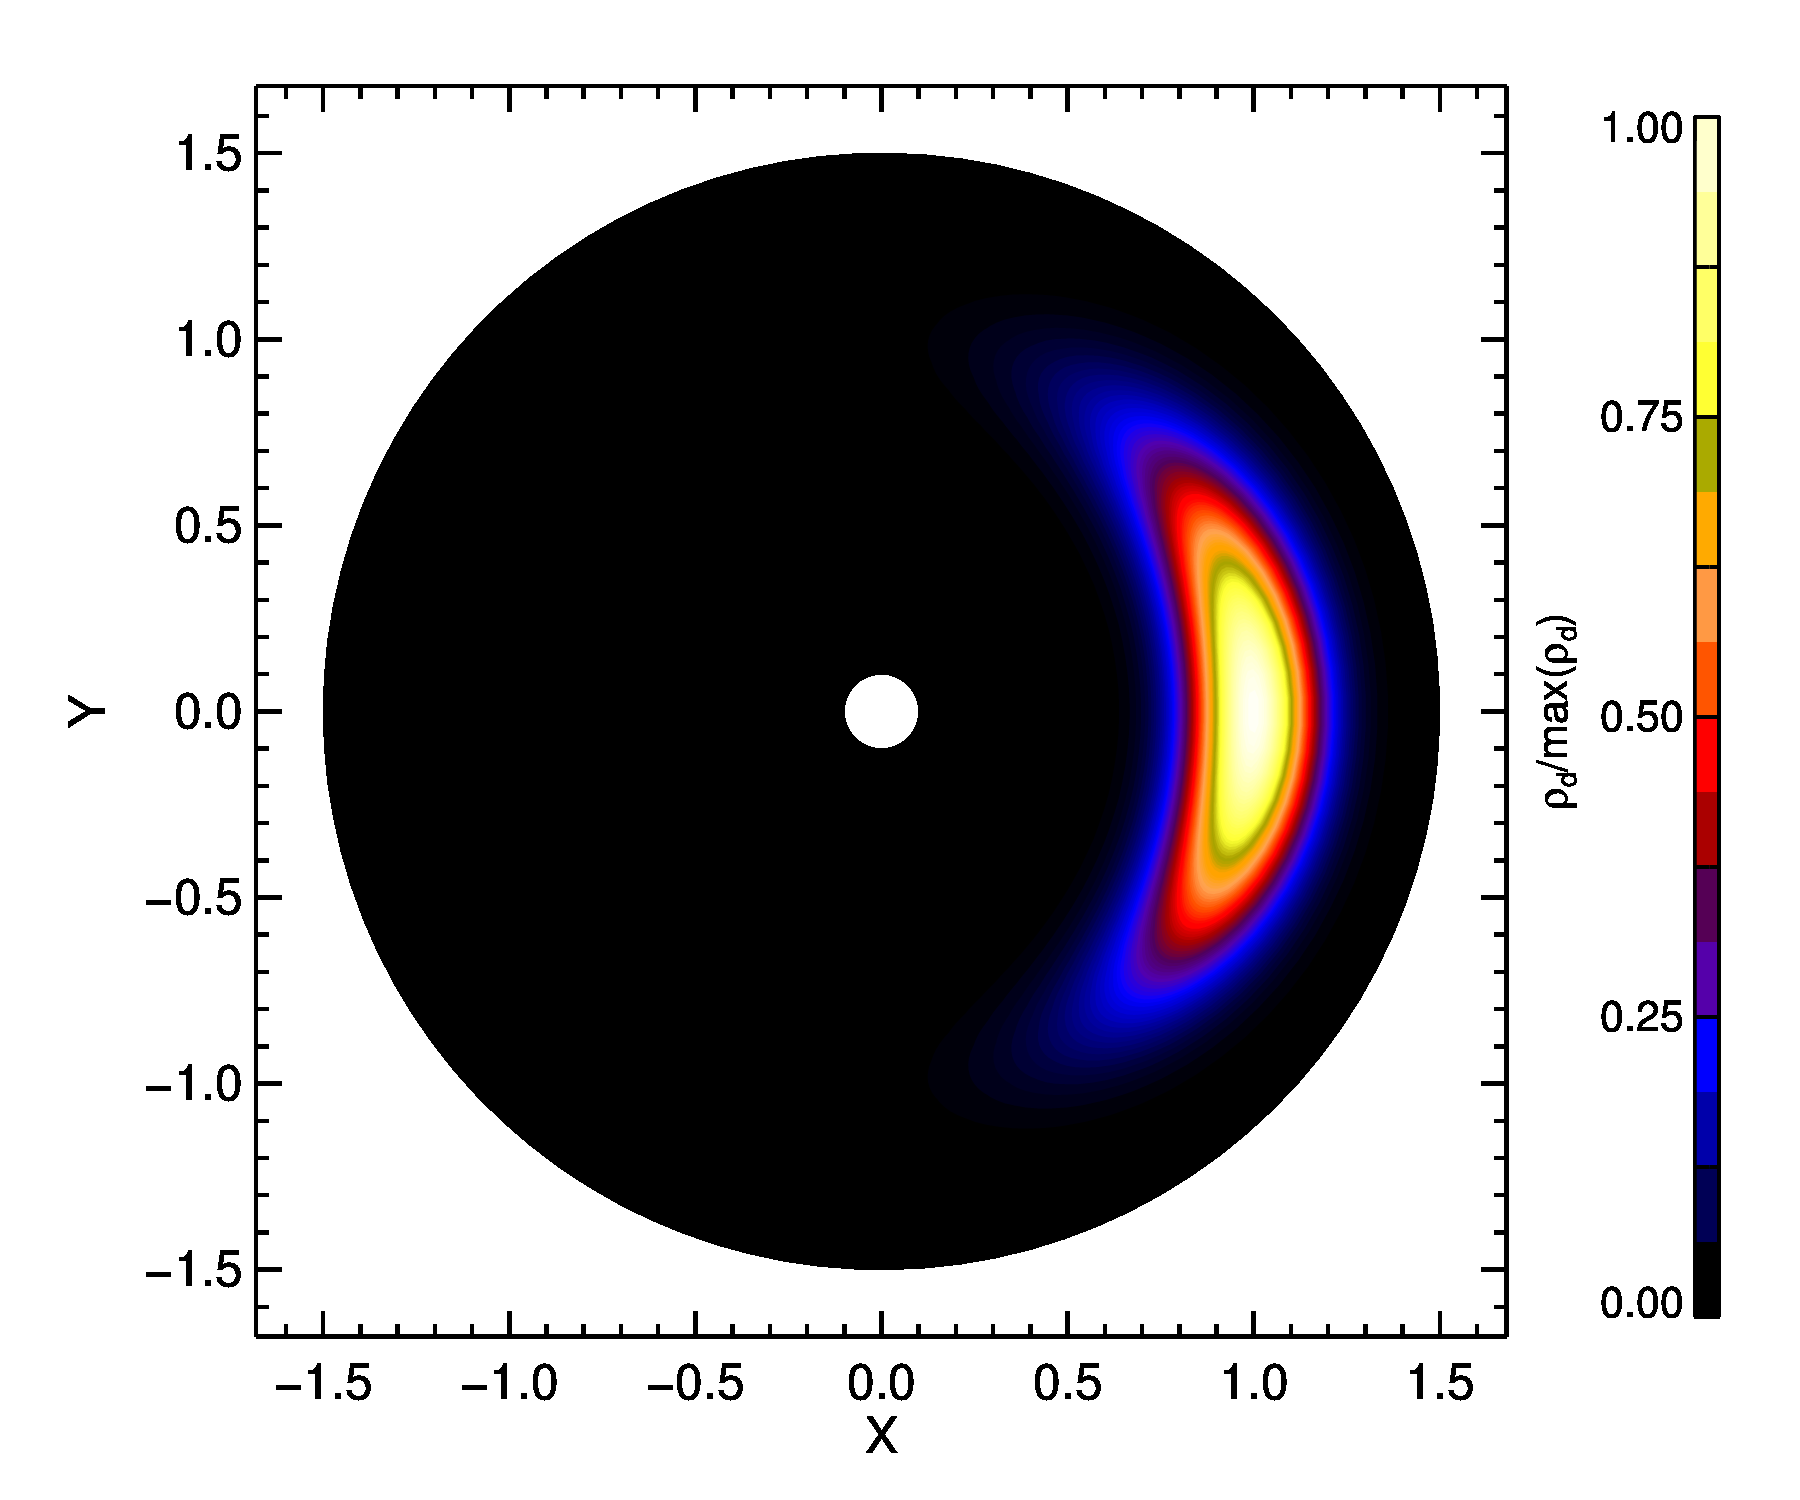
\includegraphics{../figs/disk.png}}
 \end{center}
\caption[]{Three parameters, plus a vortex solution, control the dust distribution. 
The figure shows the appearance of the dust trapped in a Kida vortex of $\chi=4$, 
for \blue{$S$}=1, in a disk of aspect ratio $H/r$=0.1.} 
 \label{fig:disk}
\end{figure}

\begin{figure}
  \begin{center}
    \resizebox{\columnwidth}{!}{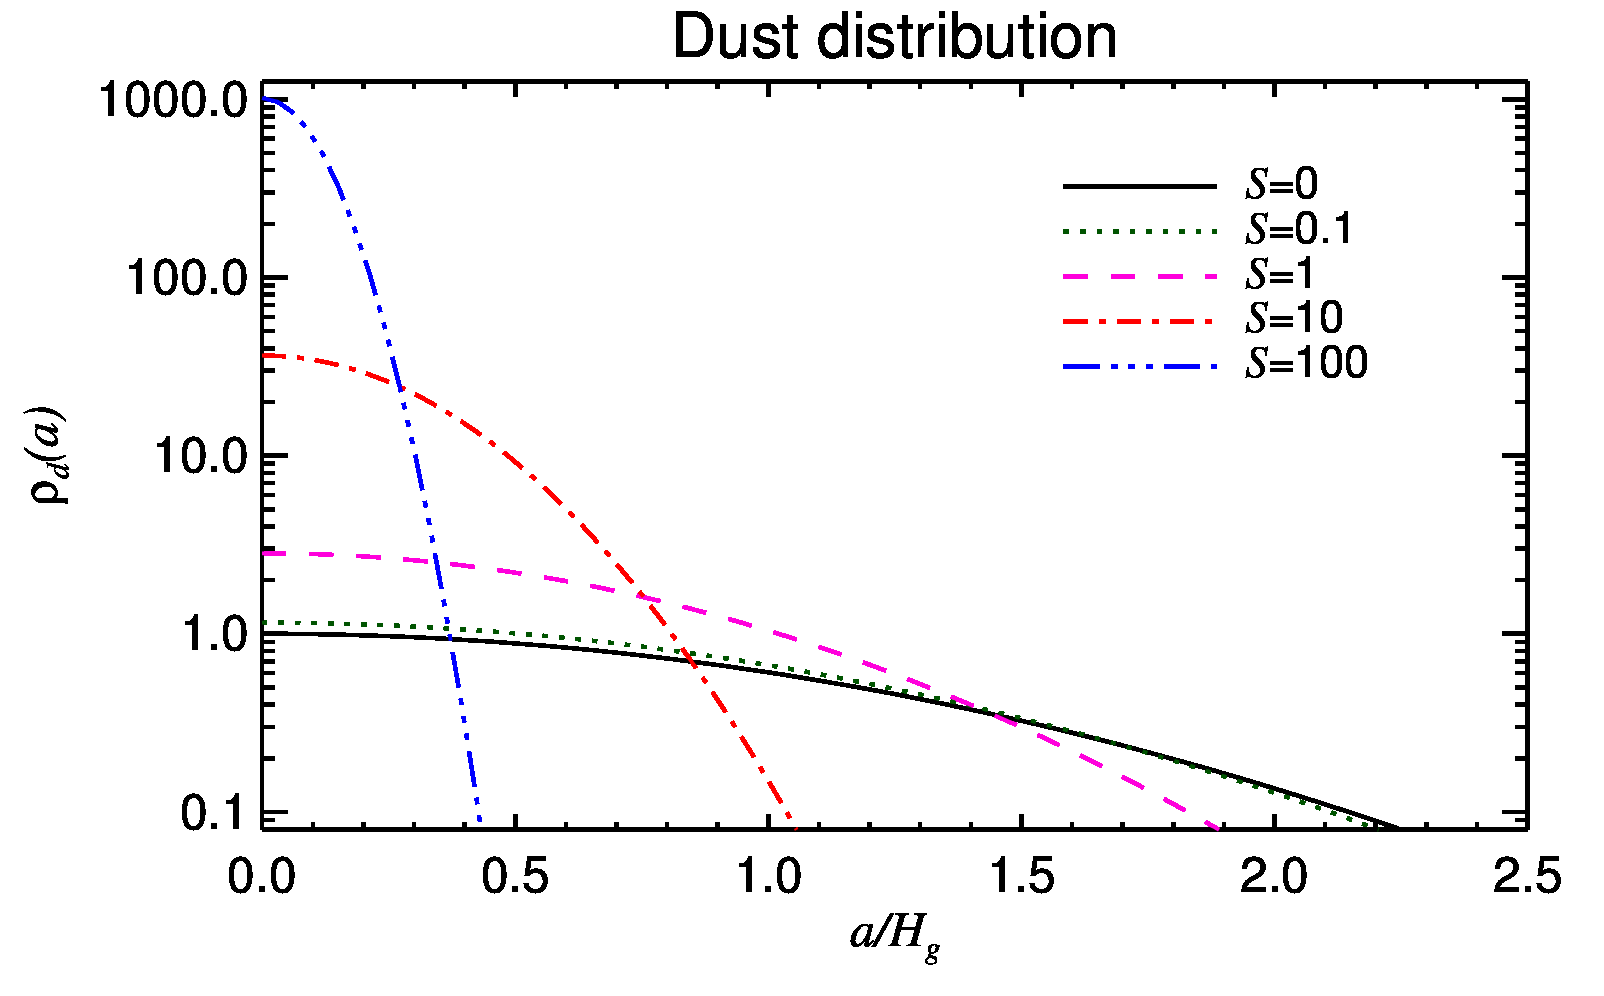
\includegraphics{../figs/gaussian.png}}
  \end{center}
\caption[]{Dust distribution for the ``axisymmetric'' case \blue{(in
    the coordinate system defined by \eqs{eq:change-x}{eq:change-y})}. \blue{The
    maximum density is proportional to $(S+1)^{3/2}$}. Curves for
  \blue{$S$}=\blue{0,} 0.1, 1, 10, and \blue{100} are shown. \blue{The
  $S$=0 case represents tracer particles and, consequently, the gas
  density. The $x$-axis is $a/H_g$, where $H_g=H/f(\chi)$ is the
  vortex scale length in the gas phase, with $H$ the sonic scale and
  $f(\chi)$ the model-dependent scale function
  \eqp{eq:scale-function}.}}
 \label{fig:gaussian}
\end{figure}


%\subsection{Axisymmetric $\v{u} = \v{v}$ }
%It is illustrative to consider the case in which $|\v{u}| \gg \tau|\grad{h}|$,
%so that we can approximate $\v{v}=\v{u}$ in the advection term\red{.} (We do
%not make this substitution in the compression term because $\v{u}$ is
%exactly divergence-free). In this case, \eq{eq:dust-trapping-uvzero} reduces
%to a relatively simple equation 
%\beq\label{eq:uveq}
%\left(\Laplace{} + A\partial_\nu + B \right)\rho_d = 0. 
%\eeq
%\eq{eq:uveq} reflects dust diffusion (first term), dust advection due
%to the vortex flow (second term) and dust concentration (third term). 
%Note that we are effectively considering regions close to the vortex
%center because $\nabla h$ vanishes at the origin, while $\nabla^2h$
%(i.e. $B$), does not.   
%Now, assuming axis-symmetry and integrating in
%$\frac{1}{2\pi} \int_0^{2\pi} d\nu$, we get  
%\beq
%\frac{\epsp}{2}\pderivn{\rho_d}{a}{2} +
%\frac{\epsp}{2a}\pderiv{\rho_d}{a} + B \rho_d = 0.  
%\eeq
%That is, 
%\beq
%y^{\prime\prime} + \frac{1}{a}y^\prime + k^2 y = 0. 
%\label{eq:axisymmetric}
%\eeq where $y(a) = \rho_d$ and $k$ is given by \eq{eq:k}. 
%\eq{eq:axisymmetric} only differs from \eq{eq:dust-trapping-axis} through the
%absence of the $k^2a\partial_a$ term, which appears when the full
%expression for the dust velocity is used consistently, and that term represented
%axisymmetric advection, which is entirely absent in the 
%problem here. Physically, as $a\to0$ there is no advection, so the two
%equations behave similarly, both stating a balance between dust
%concentration and dust diffusion. 
%%
%The general solution of \eq{eq:axisymmetric} is a
%sum of Bessel functions of the first and second kinds: 
%\beq
%y(a) = c_1 J_0 (ka) + c_2 Y_0(ka). 
%\eeq
%\noindent Since  $Y_0$ diverges at the origin, we can physically discard 
%this solution, setting $c_2=0$. So, the axisymmetric mode is $\rho_d(a)
%= c_1 \ J_0 (ka)$, or
%\beq
%\rho_d(a) = c_1 \ J_0 \left(\frac{a}{H} \ f(\chi) \sqrt{\frac{2\St}{\delta}}\right).
%\eeq 
%The Bessel function $J_0(x)$ is
%non-monotonic, with the first root around $x=2.5$. The first zero is therefore around
%$a_0 \approx H \sqrt{\delta/\St}$.  As the density
%cannot be negative, that sets the validity of our solution. 
%The solution is also constrained by our use of the shearing sheet
%equations, so the results should not be valid for $x \gg H$.
%As we made use of the approximation $\v{v}=\v{u}$, $\St \ll 1$,
%and the solution  is indeed $a_0 \gg H$, for finite values of $\delta$.
%%
%We compare in \fig{fig:bessel-gaussian} the Bessel function with the exponential found in the
%previous section for the general solution. They agree up to 10\% inside
%$ka$=1.5 (i.e., $a/H_V\approx 1$), and up to 1\% within $ka$=1 (i.e.,
%$a/H_V\approx 0.7$). Confident that approximating $\v{u}=\v{v}$ for
%advection works well within the vortex core, we use this
%simplification to find solutions to the full non-axisymmetric problem,
%in the next section. 
%
%\begin{figure}
%  \begin{center}
%    \resizebox{\columnwidth}{!}{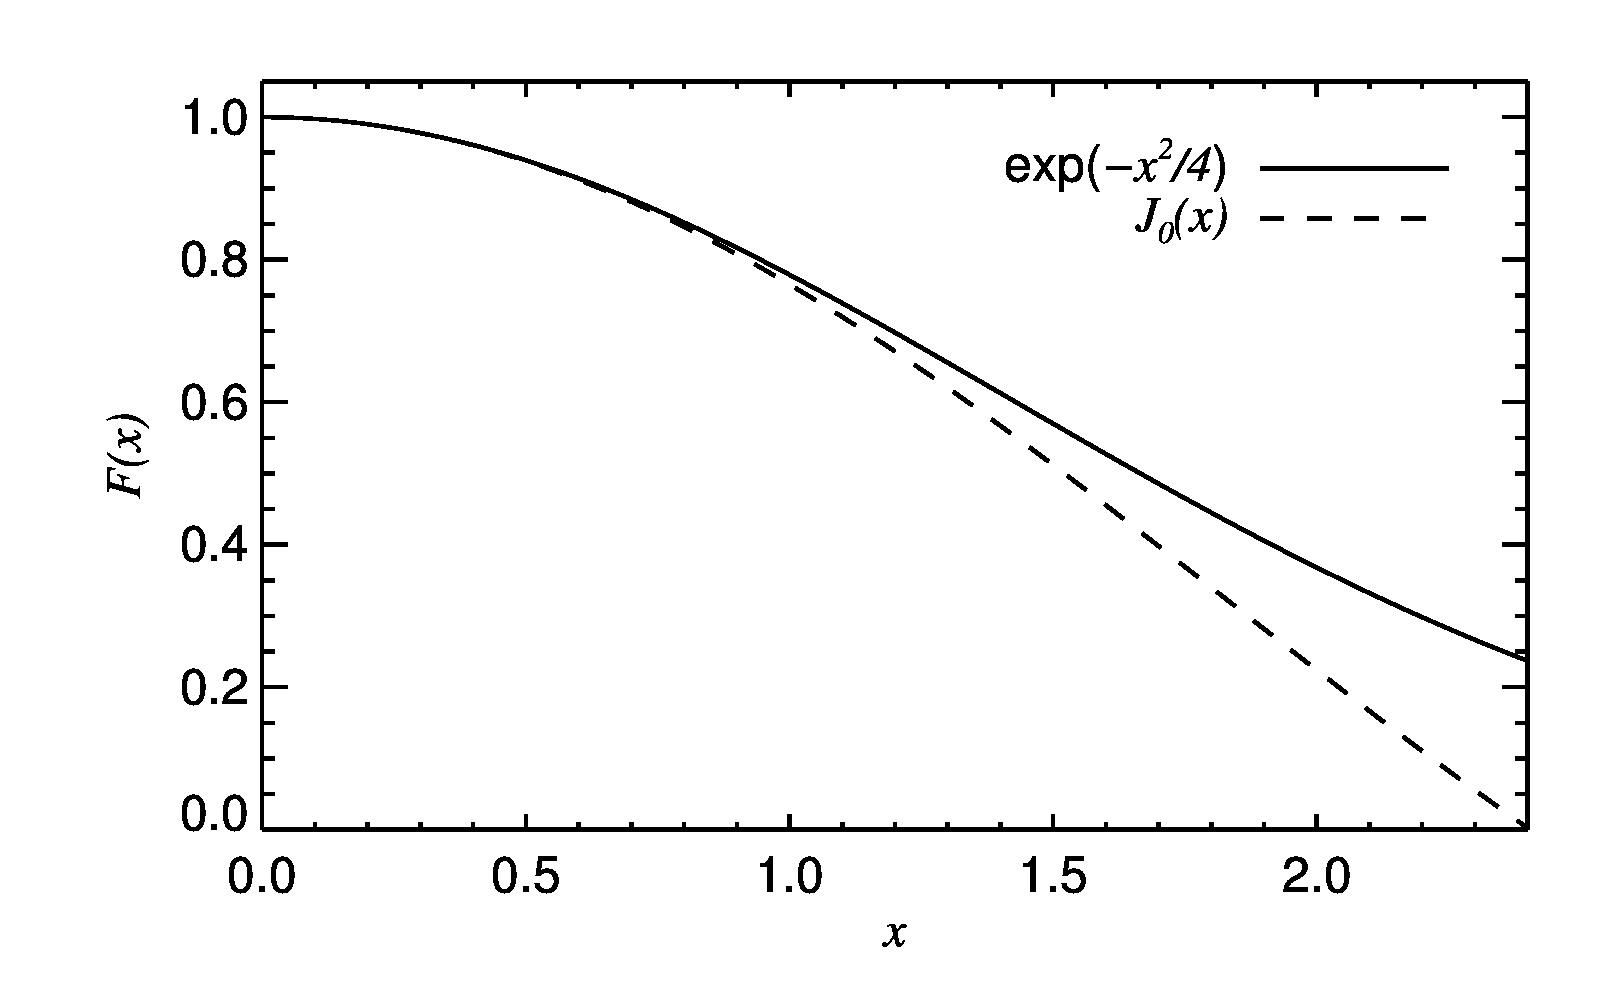
\includegraphics{../figs/bessel-gaussian.png}}
%  \end{center}
%\caption[]{The axisymmetric solutions for (solid line) the general 
%$\v{v}=\v{u}+\tau\grad{h}$ case and, (dashed line) the case where
%  we set $\v{v}=\v{u}$ for dust advection. 
%The exponential and Bessel solutions agree up to 10\% up to $x$=1.5, and up 
%to 1\% up to $x$=1. This means that dust advection due to $\tau\nabla{h}$
%is not significant within $x\lesssim1$. We conclude that the latter
%approximate solution is quite accurate for describing the dust
%distribution in the vortex core.} 
% \label{fig:bessel-gaussian}
%\end{figure}


\section{Non-axisymmetric corrections}
\label{sect:nonaxisymmetric} 

We \blue{now} consider the non-axisymmetric problem ($\partial_\nu\neq0$)\blue{.} 
We explicitly show that such effects are small 
\blue{in the vortex core} provided the \blue{effective} Stokes number \blue{$\overline{\mathrm{St}}\equiv\mathrm{St}+\delta$} is not large. \blue{These requirements will become
apparent as we proceed through the solution method. In this section we
consistently refer to ``axisymmetric'' as $\nu$-symmetry in the coordinate
system defined by \eqs{eq:change-x}{eq:change-y}.} 


\subsection{Conversion to ordinary differential equations}

The dust density $\rho_d$ is periodic in the $\nu$ co-ordinate. We 
therefore seek solutions of the form

\beq\label{eq:series-n}
\rho_d(a,\nu) = {\rm Re}
\left[\sum_{n=0}^\infty\rho_n(a)\exp{\left(\mathrm{i}n\nu\right)} \right].
\eeq

For convenience, we will drop the real part notation from now on. Inserting
\eq{eq:series-n} into the partial differential equation \eqp{eq:dust-trapping-uvzero},
multiplying by $\exp{(-\mathrm{i}m\nu)}$, and integrating the resulting
expressions over the $\nu$ co-ordinate, we arrive at a set of coupled
ordinary differential equations, 

\blue{
\beq\label{eq:ode2}
\mathcal{B}_m\rho_{m-2} (\blue{\zeta})+ \mathcal{A}_m\rho_m(\blue{\zeta}) + \mathcal{C}_m\rho_{m+2}(\blue{\zeta}) = 0,
\eeq
}
where $\blue{\zeta}\equiv ka$, and

\beqn
\mathcal{B}_m &\equiv& \blue{\tilchi}\frac{d^2}{d\blue{\zeta}^2} + \left[\blue{\beta \blue{\zeta}}-
  \frac{2\blue{\tilchi}}{\blue{\zeta}}
  \left(m-\frac{3}{2}\right)\right]\frac{d}{d\blue{\zeta}}+\left(m-2\right)\left(\frac{m\blue{\tilchi}}{\blue{\zeta}^2}\blue{-\beta}\right), \notag\\
&&\label{eq:ops}\\ 
\mathcal{A}_m&\equiv&\frac{d^2}{d\blue{\zeta}^2} +\left(\frac{1}{\blue{\zeta}}\blue{+\frac{\blue{\zeta}}{2}}\right)\frac{d}{d\blue{\zeta}} +\left(k_m^2-\frac{m^2}{\blue{\zeta}^2}\right),\\
%
&&\notag\\
\mathcal{C}_m &\equiv& \blue{\tilchi}\frac{d^2}{d\blue{\zeta}^2}
+\left[\blue{\beta \blue{\zeta}} +
  \frac{2\blue{\tilchi}}{\blue{\zeta}}\left(m+\frac{3}{2}\right)\right]\frac{d}{d\blue{\zeta}}
+ \left(m+2\right)\left(\frac{m\blue{\tilchi}}{\blue{\zeta}^2}
  \blue{+\beta}\right),\notag\\
&&\label{eq:opsw}
\eeqn
where \blue{$\tilchi\equiv(\chi^2-1)/[2(\chi^2+1)]$}, $k_m^2 \equiv 1+\mathrm{i}mA/B$\blue{, and}
\beq
\blue{\beta \equiv \frac{B_1-B_2}{2k^2(1+\chi^{-2})} = \frac{B_1 - B_2}{4B}.}
\eeq
%[Recall $k^2\equiv 2B/\left(1+\chi^{-2}\right)$.] The independent variable is $\blue{\zeta}\equiv ka$. 
\blue{Note that $\beta$ is a function of the aspect-ratio depending on the vortex model.} 
\eq{eq:ode2} holds for each $m$ except for $m=0$ for which the $\rho_{m-2}$ terms are absent. Each 
$\rho_m$ couples to $\rho_{m\pm2}$ through operators $\mathcal{B}_m$
and $\mathcal{C}_m$. The axisymmetric problem is recovered by
setting $\rho_{m>0}=0$. 

\blue{We} expect $\rho_d(a,\nu)$ to have even symmetry in
$\nu$ \blue{because of the elliptical nature of the vortex streamlines}. 
Henceforth we only consider even $m$. We seek solutions with  
$\rho_m^\prime(0)=0$ \blue{(where the prime denotes derivative with respect to the argument)} and $\rho_{m\geq2}(0)=0$, so that
$\partial_x\rho_d=\partial_y\rho_d=0$ at the origin, consistent with 
dust reaching maximal density there.  

\blue{\subsection{Operator properties}}

\blue{
Consider 
\begin{align}
	g_m(\blue{\zeta}) \equiv \blue{\zeta}^m\exp{(-\blue{\zeta}^2/4)}.
\end{align}
Then we find that 
\beqn
\mathcal{B}_mg_{m-2} &=&\frac{1}{4}\left(\tilchi - 2\beta\right)g_m,\\
\mathcal{A}_mg_m &=& \left(k_m^2 - \frac{m}{2} - 1\right)g_m,\\
\mathcal{C}_mg_{m+2}&=& \left[4\tilchi(m+1)(m+2) +2(\beta-\tilchi)(m+2)\blue{\zeta}^2 \right.
\notag\\ &+&\left. \frac{\left(\tilchi - 2\beta\right)}{4}\blue{\zeta}^4\right]g_m. 
\eeqn
The first two expressions will be useful in constructing nearly-axisymmetric solutions. 
}

\blue{
\subsection{Exact axisymmetric solutions}
It is useful to see how the formulation above connects with the  axisymmetric solutions discussed in the previous section.  Consider the special case where $\tilchi = 2\beta$, so that 
%\begin{align}
$\mathcal{B}_mg_{m-2} = 0.$
%\end{align}
Then the complete solution to \eq{eq:ode2} is $\rho_0 = b_0e^{-\blue{\zeta}^2/4}$ with $\rho_{m>0} \equiv 0$, and $b_0$ is an arbitrary constant. That is, if $\tilchi=2\beta$ then the dust distribution is exactly axisymmetric. 
}
\blue{
\subsubsection{Dust in a GNG vortex is axisymmetric}
For the GNG vortex, one can verify that $\tilchi\equiv 2\beta$, implying dust density only depends on the ellipse under consideration, not the position along it. This is because the GNG vortex has no pressure gradient along the elliptical streamlines \citep{Chang-Oishi10}. 
}
\blue{
\subsubsection{Condition for dust in a Kida vortex to be axisymmetric}
For the Keplerian Kida vortex, we find
\begin{align}
\tilchi - 2\beta = \frac{\chi(\chi-1)(\chi-7)}{2(\chi-2)(2\chi+1)(\chi^2+1)}.
\end{align}
The dust distribution is exactly axisymmetric for aspect-ratio $\chi=7$, which is also when the Keplerian Kida vortex has no pressure gradient along its elliptical streamlines \citep{Chang-Oishi10}. 
}
\blue{
\subsection{Source term approximation}
In preparation for constructing non-axisymmetric solutions, we here describe the \emph{source term approximation} \citep{Zhang06}.
We assume that $|\rho_m|$ decreases with $m$, so that in \eq{eq:ode2} the $\mathcal{C}_m\rho_{m+2}$ term has smallest magnitude.  Neglecting it as a first approximation, we solve 
}
\blue{
\begin{align}
\mathcal{A}_m\rho_m = \begin{cases}
        0 & m =0 \\
	-\mathcal{B}_m\rho_{m-2} & m \geq 2.
\end{cases}
\end{align}
The solutions are 
\begin{align}\label{eq:series1}
\rho_m (\blue{\zeta})= b_m g_m(\blue{\zeta}),
%\begin{align}\label{eq:series}
%\rho_m (\blue{\zeta})= b_m \blue{\zeta}^m\exp{(-\blue{\zeta}^2/4)}, 
\end{align}
with
\begin{align}
b_m  = -\frac{\left(\tilchi - 2\beta\right)}{2\left[2k_m^2 - (m+2)\right]}b_{m-2}
\end{align}
for $m\geq2$, and $b_0$ is arbitrary as before. Note that $b_m=0$ for odd $m$ because $b_1=0$ since 
we require $\rho_1^\prime(0)=0$. Then, by induction 
\begin{align}\label{eq:induction}
b_m  = \left(-1\right)^{m/2}\frac{\left(\tilchi/2-\beta\right)^{m/2}}{\prod_{l=1}^{m/2}
\left(2k_{2l}^2 -2l - 2\right)}b_0,
\end{align}
for even $m\geq 2$.  
}

\blue{
The source term approximation assumes 
$R\equiv|\mathcal{C}_m\rho_{m+2}|/|\mathcal{A}_m\rho_m| \ll 1.$ 
For given $\blue{\zeta}$, the solution $\rho_m=b_mg_m$ is consistent with this requirement if $|k_m^2|\gg1$, corresponding to small effective Stokes number.  
 However, this approximation will eventually fail for large $\blue{\zeta}$ because the solution above implies $R\propto \blue{\zeta}^4$ for $\blue{\zeta}\gg1$. Thus the solution is only self-consistent for sufficiently small $\blue{\zeta}$ and/or $\overline{\St}$. Nevertheless,
we comment that the closed-formed solutions obtained here may be useful in
an iterative scheme to obtain numerical solutions to the full set of ODE's. 
}

\blue{
\subsection{Weakly non-axisymmetric dust distributions}
We are now ready to construct non-axisymmetric solutions. 
%The previous results indicate the axisymmetry is possible if there is no pressure gradients along the ellipse. 
Consider a Keplerian Kida vortex with $\chi\neq 7$, meaning that the effective 
frictional force on the dust has a non-vanishing component along the
fluid velocity vector. (I.e. dust particles are accelerated along the
ellipse.) We assume non-axisymmetry in the dust distribution is
sufficiently weak, so one may truncate the series solution at
$m=2$. Thus we set $\rho_{m>2}\equiv0$.} Let
\begin{align}
\rho_0(\blue{\zeta}) = b_0\blue{g_0(\blue{\zeta})} + \epsilon(\blue{\zeta}),
\end{align}
where $\epsilon(x)$ represents the correction to the axisymmetric
solution due to $\rho_2(\blue{\zeta})$. The ODEs to be solved are

\begin{align}
&\mathcal{A}_0\epsilon(\blue{\zeta}) = -\mathcal{C}_0\rho_2(\blue{\zeta}),\label{eq:m2_eq1}\\
&\mathcal{A}_2\rho_2(\blue{\zeta})   = \blue{-\mathcal{B}_2\left(b_0g_0 + \epsilon\right)}.\label{eq:m2_eq2}
\end{align}
To make further progress, at this stage we \emph{assume} that the
$\epsilon$ term in Eq. \ref{eq:m2_eq2} can be neglected\blue{, so $\rho_2 = b_2 g_2$ with $b_2$ given by the source term approximation.} 
This means that  

\blue{
\beq\label{eq:rho2}
\frac{\rho_2}{\rho_0} = \frac{b_2}{b_0}\blue{\zeta}^2,
\eeq
}
\blue{
implying non-axisymmetry becomes significant for sufficiently large $\blue{\zeta}$, 
and truncating the series at $m=2$ is no longer self-consistent. 
%(higher $m$ components should be included) 
However, in practice the ratio $|b_2/b_0|$ is small. 
For example, inserting $\chi=4$ gives $|b_2/b_0|\simeq0.1\%$ for
$\overline{\St}=0.1$ and $|b_2/b_0|\sim 1\%$ for $\overline{\St}=1$. Since
most of the dust is contained within $\blue{\zeta}\lesssim 1$, we conclude that
non-axisymmetry is {\it in general} a small effect.}

We can use \eq{eq:rho2} in \eq{eq:m2_eq1} to
calculate the correction term $\epsilon$. We find

\beq
\epsilon(\blue{\zeta}) = \blue{\frac{1}{8}b_2g_2\left[-16\tilchi+\left(\tilchi - 2\beta\right)\blue{\zeta}^2\right]}.
\eeq

Collecting the above results and Taylor-expanding the \blue{$g_m$}'s, our
weakly non-axisymmetric solution for $\blue{\zeta}\ll 1$ reads:

\begin{align}
&\rho_0(\blue{\zeta}) =1 -  \frac{\blue{\zeta}^2}{4}\left[1-\frac{\tilchi\left(\tilchi \blue{- 2\beta}\right)}{\mathrm{i}A/B \blue{- 1/2}}\right]+ O(\blue{\zeta}^4),\\
&\rho_2(\blue{\zeta}) =-\frac{\left(\tilchi \blue{- 2\beta}\right)}{2\left(4\mathrm{i}A/B \blue{- 2}\right)}\blue{\zeta}^2+O(\blue{\zeta}^4)
\end{align}
where we have used the definition of $k_m$ \blue{and set $b_0=1$
  without loss of generality}. %We see that non-axisymmetric effects
%are weak for $\mathrm{St}\ll1$ because $B\propto \mathrm{St}$.  
In the previous section, we obtained the axisymmetric solution
assuming the \blue{non-}axisymmetric components are negligible. 
Here, we see explicitly that the axisymmetric solution in fact leads
to non-axisymmetry through the coupling terms, but these corrections
are small for $\overline{\St} \ll 1$, because $B \propto \overline{\St}$. We conclude that dust in the vortex core is effectively axisymmetric.
%This makes sense because the force on the dust along the ellipse is proportional to $\mathrm{St}$. 

\subsubsection{Consistency check}
Using the above expression for $\epsilon(\blue{\zeta})$, we can evaluate
$\mathcal{B}_2\epsilon(\blue{\zeta})$ in order to assess our assumption that
$\epsilon(\blue{\zeta})$ has a negligible contribution to $\rho_2$. We find

\beqn
\mathcal{B}_2\epsilon(\blue{\zeta}) =&& \blue{\left[32\tilchi(5\tilchi - 6\beta)-16(\tilchi-2\beta)(2\tilchi-\beta)\blue{\zeta}^2
\right.\notag}\\&&\blue{\left.+(\tilchi - 2\beta)^2\blue{\zeta}^4\right]\frac{b_2g_2}{32}.}
\eeqn

Provided that $|k_2^2|\gg1$ \blue{and $\blue{\zeta}$ is not large},  
this term is indeed small compared to the first term on the RHS of \eq{eq:m2_eq2}.  \blue{For example, considering $\blue{\zeta}=1$, 
for $\chi=4$ and $\overline{\St}=0.1$ we obtain $|\mathcal{B}_2\epsilon|/|\mathcal{B}_2\rho_0|\simeq0.02$. 
Even with $\overline{\St}=1$, this ratio $\sim0.2$ is not large. We
conclude that}  our solution procedure above is self-consistent.

\section{\blue{Observational predictions}}
\label{sect:observables}

\blue{Having arrived at the ``axisymmetric'' solutions (in the
  $a$-$\nu$ plane, \sect{sect:axisymmetric}), and shown that deviations from
  $\nu$-symmetry are small (\sect{sect:nonaxisymmetric}), we go back to
  the solutions of \sect{sect:axisymmetric} to derive observational predictions.}

\blue{\subsection{Dust - gas contrast}}

\blue{\eq{eq:gen_axi} and \eq{eq:gas_axi} also allows us to calculate the gas-dust
density contrast, and, therefore, $\rho_{d\,{\rm max}}$ as a function of
$\rho_{g\,{\rm max}}$. For that, we calculate the volume integral of $\rho_d$
and $\rho_g$. These, in turn, need the dependencies on the vertical
coordinates $z$. These are straightforward, being $\exp(-z^2/2H^2)$ for the gas and
$\exp(-z^2/2H_d^2)$ for the dust, with $H_d=H/\sqrt{(1+S)}$ \citep{Dubrulle95}. Integrated over plus and minus infinity, these yield $\sqrt{2\pi}H$ and
$\sqrt{2\pi}H_d$, respectively. We have thus}

\blue{
\beqn
\int\rho_d(a,z) dV  &=& \rho_{d\,{\rm max}} \ \frac{(2\pi)^{3/2}}{\sqrt{S+1}} H \int_0^\infty {\rm  e}^{-a^2/2H_g^2 \ (S+1)} \ a\chi \ da \notag\\
&&= \rho_{d\,{\rm max}} \ \left(\frac{2\pi}{S+1}\right)^{3/2} \chi H H_g^2, \label{eq:integral-dust}\\ 
%
\int\rho_g(a,z) dV  &=& \rho_{g\,{\rm max}} \ (2\pi)^{3/2} H \int_0^\infty {\rm e}^{-a^2/2H_g^2} \ a\chi \ da\ \notag\\
 &&= \rho_{g\,{\rm max}} \ (2\pi)^{3/2} \chi H H_g^2. \label{eq:integral-gas}\\
\eeqn 
\noindent Dividing \eq{eq:integral-dust} by \eq{eq:integral-gas}, the
ratio of the integrals in the left hand sides is the global dust-to-gas
ratio, $\varepsilon$. The density enhancement factor is thus
\beq
  \rho_{d\,{\rm max}} =  \varepsilon \ \rho_0 \ (S+1)^{3/2} \label{eq:maxrhod}
\eeq where $\rho_0=\rho_{g\,{\rm max}}$ is an appropriate reference
density. The full expression for the dust density is therefore} 

\blue{\beq
   \rho_d(a,z) = \varepsilon \, \rho_0 \, (S+1)^{3/2} \  \exp{\left\{-\frac{\left[a^2f^2(\chi) + z^2\right]}{2H^2}(S+1)\right\}} 
\label{eq:sect6-exp}
\eeq}

\blue{\eq{eq:maxrhod} shows that the dust-to-gas ratio at the origin (vortex center)
is related to the total dust-to-gas mass ratio by a simple function of $S$.  
In this enhancement, only a third (in log) is caused by sedimentation. The
rest is due to in-plane vortex capturing. Midplane dust
distributions for different values of \blue{$S$} are plotted in \fig{fig:gaussian}, as a 
function of $a/H_g$.} 

\blue{\subsection{Trapped mass}}

\blue{For the total trapped mass, we simply need
to integrate \eq{eq:sect6-exp}, which amounts to replacing
\eq{eq:maxrhod} in \eq{eq:integral-dust}
 \beq
\int\rho_d(a,z) dV  = \left(2\pi\right)^{3/2} \, \varepsilon \, \rho_0 \ \chi H H_g^2 \label{eq:dust-mass}\\ 
\eeq
}

\blue{\subsection{Dust density contrast}}

\blue{The contrast in the same orbit is found by calculating the
  minimum dust density and comparing it to \eq{eq:maxrhod}. By substituting the gas solution \eqp{eq:gas_axi}
  into \eq{eq:gen_axi} we can write
\beq
\frac{\rho_{d\,{\rm max}}}{\rho_{d\,{\rm min}}} = \frac{\rho_{g\,{\rm max}}}{\rho_{g\,{\rm min}}} \exp{(S)},\label{eq:max-contrast}
\eeq
which is the same result
as found by \cite{Birnstiel13}, provided a suitable choice is made for
$\delta$ (we do not assume a relationship between $\delta$ and $\alpha$
because the turbulence in the vortex core is locally generated and
unrelated to the disk turbulence, c.f., elliptic instability,
\citealt{Lesur-Papaloizou10,Lyra-Klahr11}).
%
 The minimum densities occurs at the boundary of the vortex, which is
 the sonic perimeter where shocks occur. Its limit is found by
 writing the vortex velocity \eqp{eq:vortex} as a Mach number 
\beq
  {\rm Ma} = \frac{|u_y|}{c_s} = \omega_V\chi \  \frac{x}{H} 
  \label{eq:vortex-mach}
\eeq and setting ${\rm Ma} = 1$. This yields the
boundary at 
\beq
a_s = H (\chi \omega_V)^{-1} \label{eq:sonic}
\eeq where the subscript $s$ stands for
sonic. The Kida solution asymptotically reaches $a_s=2H/3$, while the
GNG solution asymptotically reaches $a_s=H/\sqrt{3}$. In the physical
range of relevance ($2\lesssim \chi \lesssim 10$), they both yield values around $H/2$, which matches  
the results of numerical simulations. Substituting \eq{eq:sonic} in \eq{eq:gas_axi}, the gas density contrast is 
\beq
  \frac{\rho_{g\,{\rm max}}}{\rho_{g\,{\rm min}}} =
  \exp{\left[\frac{f^2(\chi)}{2\chi^2\omega_V^2}\right]}, \label{eq:gas-contrast}
\eeq
\noindent For neither the Kida nor the GNG solutions does this quantity
deviate much from unity. This is because the argument in the exponent tends
asymptotically in both cases to small fractions of $f^2$; $2/9$ in the
Kida case, $1/6$ in the GNG case.} 

%which translates into a contrast of $\approx$2.16 for a Kida
%vortex, and $\approx$1.56 for a GNG vortex. 

\blue{\subsection{Measuring $\delta$}}

\blue{Closed elliptic streamlines are subject to the elliptic
instability, which leads to subsonic turbulence in the vortex core 
\citep{Lesur-Papaloizou10,Lyra-Klahr11}. To directly measure $\delta$, 
the turbulent diffusion parameter, one would need to measure the 
turbulent velocity field. As $\alpha$, the Shakura-Sunyaev viscosity
parameter \citep{Shakura-Sunyaev73}, $\delta$ can be
defined as the ratio of stress over pressure. If the turbulence is
isotropic in the midplane, one can write 
\beq
\delta = v_{\rm  rms}^2/c_s^2,
\eeq where $v_{\rm rms}$ is the rms of the turbulent velocities. 
The beam smearing would render the velocity field 
unresolved even for moderately close systems, so one should 
look for unresolved signatures. Spectroscopically, this extra rms velocity should have 
an effect similar to microturbulence, providing an slight extra
broadening to the Doppler core of suitable spectral lines.}

\blue{For gas temperatures ranging 20-200\,K, assuming that the gas is a 5:2 hydrogen to
helium mixture (mean molecular weight of 2.4), the isothermal sound
speeds range 0.26-0.83 \, km/s. Considering that typical velocities of subsonic
turbulence are $\approx$10\% of the sound speed ($\delta \approx
10^{-2}$), the typical velocity signal for 200\,K would of the order
of $\leq$0.1\,km/s. As \cite{vanderMarel13} quote a
sensitivity limit of ALMA of 0.2\,km/s for their observations of
Oph IRS 48 only the $\geq$2$\sigma$ tail of the turbulent velocity field
would be detectable.} 

\blue{If a direct determination of $\delta$ does not sound promising,
  an indirect way is possible by measuring $S$ and $\St$. The
  parameter $S$ can be determined via the dust-density
  contrast with \eqs{eq:max-contrast}{eq:gas-contrast}, or via the
  dust-gas contrast at maximum \eqp{eq:maxrhod}. The Stokes number is 
\beq
    \St = \tauf  \varOmega = \sqrt{\frac{\pi}{8}} \
    \frac{a_\bullet}{H} \ \frac{\rho_\bullet}{\rho_g}
\eeq
\noindent where $a_\bullet$ is the particle radius and $\rho_\bullet$ the
particle internal density.} 

%\blue{\section{Limitations}}

%%%%%%%%%%%%%%%%%%%%%%%%%%%%%%%%%%%%%%%%%%%

% 30 mili-arcseconds. spatial resolution

\blue{\subsection{Application to Oph IRS 48}}

\blue{We now apply our model to the observed Oph IRS 48 system, with the
parameters derived by \cite{vanderMarel13}.The dust contrast in the same orbit is 130, which, according to
\eq{eq:max-contrast} and \eq{eq:gas-contrast} for $\chi=3.1$, set $S=4.79$ and
$S=4.82$ for the Kida and GNG solutions, respectively.  The values are
close because the gas contrast is small \eqp{eq:gas-contrast}.}

\blue{The dust temperature is estimated at 60\,K. Assuming this is the
  same as the gas temperature, and a mean molecular weight of 2.4, the isothermal sound speed is 
  $c_s \approx {\rm 456 \, cm/s}$. At $r_0$=63\,AU, around a $2 M_\sun$ star, this translates into an aspect
  ratio of $H/r \approx0.09$, or $H\approx5.4$ \,AU. The particle radius measurement is $a_\bullet \approx 4$\,mm. 
The gas density is highly uncertain. \cite{Brown12} estimate the mass
as $10^{-4} - 10^{-3} M_\sun$ within 30\,AU, using a mm flux vs mass
calibration \citep{Beckwith90}, which translates into a surface
density of 10$^{15}$-10$^{16}$ \, cm$^{-2}$ assuming
H$_2$/CO=10$^4$. For a mean molecular weight of 2.4, these values imply $\rho_g \approx 3 \times 10^{-14}-10^{-15}$ g\,cm$^{\rm  -3}$. We
take the mean (in log), $\approx 10^{-14}$ g\,cm$^{\rm  -3}$, as
representative. For particles of material density 
$\rho_\bullet=0.8 g\,{\rm cm}^{-3}$, the
Stokes number should be $\St \approx 0.25$. For $S=4.8$, this translates
into $\delta \approx 5\times 10^{-2}$, meaning typical turbulent velocities in the
vortex core at $\sqrt{\delta} \approx 22\%$ of the sound speed. These
velocities are somewhat on the high side, as the speeds expected for
the elliptic instability range from 5-10\% of the sound speed
\citep{Lesur-Papaloizou10,Lyra-Klahr11}, but given the approximations,
assumptions, and uncertainties, the agreement within a factor $\approx$ 2-4 is remarkable.}

\blue{As for the trapped mass, for the typical interstellar
dust-to-gas ratio of $\varepsilon=0.01$, \eq{eq:dust-mass} yields 0.55
and  1.39\,$M_\oplus$ for Kida and GNG, respectively. A factor 16 and
6, respectively, from the measured trapped mass of 9\,$M_\oplus$.} 

\blue{Although these values seem reasonable, it should be noted that
  for Oph IRS 48 the candidate planet is at 25AU, whereas the dust trap is at 63 AU. Even though the
planet is supposed to be massive (planet-to-star mass ratio
$5\times10^{-3}$), gaps are not expected to be that wide. The supposed
vortex also seems to be very big, with a semiminor axis of 17\,AU. For
a temperature of 60\,K, this corresponds to over 3$H$, which is far
from the $\approx H/2$ expected from numerical simulations and
\eq{eq:sonic}.}

%\chi=3.1
%T=60K (assuming? typical dust temperature?) 
%mass=9 earth
%center=63
%extent:45-80 AU
%a_\bullet = up to 4 mm
%(sigmal to noise = 390)
%density constrast: 130 (same orbit)        => S=2.5
%gas density: 5x(1e-14 - 1e-15) g/cm3 

%funnybits: quartic gaussians; Sigmar = Sigmar*exp(-(r-rc)^4/2*rw^4),
%ditto for phi
%Rc=63, Rw=18 , Phic=95, phiw=50
%Mgas = 19 and 27 Jup masses of gas
%rhod=0.8 g/cm3

%The Stokes number is 

%\beq
%    \St = \tau  \varOmega = \sqrt{\frac{\pi}{8}} \ \frac{a_\bullet}{H}\frac{\rho_\bullet}{\rho_g}
%\eeq

%\noindent where a_\bullet is the particle radius and \rho_\bullet the
%particle internal density. For the possible vortex seen with 

%\rho_{d\,{\rm max}} =  \varepsilon \ \rho_0 \ (S+1)^{3/2}

% With maximum dust density
% Or turbulent broadening 
% probably maximum dust density is simpler
% (but needs to know what the gas density is, to measure the Stokes
% number)


\section{Conclusions}

We solve for the distribution of dust trapped in
disk vortices, in steady state between gas drag, that 
tends to drive dust into the vortex, and diffusion, that expels
it. \eqs{eq:gen_axi}{eq:hv}, \blue{with coefficient given by \eq{eq:maxrhod}},
 are our result for a distribution with
``axis-symmetry''  in the coordinate system defined by
\eqs{eq:change-x}{eq:change-y}. That is, consisting of ellipses of
equal aspect ratio as those of the gas vortex. The solution has some remarkable
properties. It is a Gaussian of standard deviation $H_V$, where, given
the angular velocity $\varOmega_V$ of the vortex, $H_V$
is determined by three quantities. These are: 
the sonic length and gas scale height, $H$; the vortex aspect ratio
$\chi$; and \blue{$S=\St/\delta$}, the relative strength of drag to
diffusion. The importance of this latter parameter had already been 
hinted upon by \citet{Cuzzi93} and \citet{Dubrulle95} 
in the context of steady states of dust sedimentation, and by
\citet{Klahr-Henning97} for vortices in the meridional plane. An insightful study by 
\citet{Jacquet12} emphasized the relevance of this parameter for 
global redistribution of solids. \citet{Birnstiel13} also find this to be 
the parameter of relevance in their semi-analytical model.

Transitional disks provide an interesting venue where to test the
model in an astrophysical context, since all three parameters can be
derivable from data. The vortex aspect ratio is readily observable,
and $H$ follows from the temperature ($H=c_s/\varOmega$). \blue{The 
parameter $S$ follows from the density contrast (either dust-gas
contrast at maximum or dust constrast in the same
orbit). Disentangling $\St$ from $\delta$ in this parameter requires
directly measuring at least one of these quantities. The diffusion
parameter $\delta$ is in principle not equal to
$\alpha$ (the dimensionless gas viscosity of
\citealt{Shakura-Sunyaev73}), because the processes generating turbulence in the
vortex and in the disk are different. The latter is supposedly the
magneto-rotational instability \citep[MRI,][]{Balbus-Hawley91}, whereas the former is the elliptic or
magneto-elliptic instability (see \citealt{Lyra13} and references
therein). A direct measure of $\delta$ would require measuring the
velocity field inside the vortex, that would appear spectroscopically 
as a slight extra line broadening. However, this would be
difficult because the signal is too small. Measuring $\St$ requires
knowing the gas density and temperature, the particle radius and
internal density. Of these, the internal density is difficult to measure
directly and should be inferred by laboratory experiments. We apply
the model to the Oph IRS 48 system, finding consistent values. The
Stokes number for the 4\,mm particles is estimated at 0.25, implying 
$\delta \approx 5\times 10^{-2}$. The total dust masses we estimate 
are within an order of magnitude of the measured value.}  

We also solve for the non-axisymmetric problem, \blue{showing that, for the
vortex core, it is in general but a small correction}. The solution is
\eq{eq:series-n}, with \blue{``radial'' basis functions given by
\eq{eq:series1} and} coefficients given by \eq{eq:induction}. In practice, the magnitude
of the higher non-axisymmetric modes fall fast as $m$ increases, and 
only the $m=2$ term would provide an appreciable deviation from
\blue{$\nu$}-symmetry. \blue{We find that non-axisymmetry in dust 
is associated with non-zero pressure gradients along elliptical streamlines of the vortex.}

We note that, aside from planetary gap edges, self-sustained disk
vortices may also result from RWI in the boundary between MRI-active and MRI-dead zones \citep{Varniere-Tagger06,Lyra08,Lyra09a,Lyra-MacLow12}, or
convective-like nonlinear baroclinic instabilities \citep{Klahr-Bodenheimer03,Klahr04,Petersen07a,Petersen07b,Lesur-Papaloizou10,Lyra-Klahr11,Raettig13}. 
These processes, however, are not reasonable in the context of outer
regions of transition disks: the outer edge of the dead zone is quite smooth
\citep{Dzyurkevich13,Landry13}, whereas the RWI requires a 
sharp enough transition; as for the baroclinic instability, it
requires \blue{finite thermal diffusion, whereas the thin outer disk
  is supposed to radiate efficiently}. This leaves gap-edge RWI as the only currently known
plausible mechanism to excite such vortices. 

\acknowledgments W.L. acknowledges financial support by the National Science
Foundation under grant no. AST10-09802. Part of this paper was written
at the Jet Propulsion Laboratory, California Institute of Technology, under a contract with the
National Aeronautics and Space Administration. \blue{The authors are 
indebted to J. Carpenter, N. van der Marel, J. Oishi, and L. Ricci for thoughtful suggestions. 
We thank also the anonymous referee for questions and comments that helped improve the work.} 

\begin{thebibliography}{}
\expandafter\ifx\csname natexlab\endcsname\relax\def\natexlab#1{#1}\fi

\bibitem[{{Adams \& Watkins}(1995)}]{Adams-Watkins95} Adams, F, C. \& Watkins, R. 1995, ApJ, 451, 314
\bibitem[{{Alexander et al.}(2006)}]{Alexander06} Alexander, R. D., Clarke, C. J., \& Pringle, J. E 2006, MNRAS, 369, 216
\bibitem[{{\blue{Andrews et al.}}(2011)}]{Andrews11} \blue{Andrews, S.M., Wilner, D.J., Espaillat, C., Hughes, A.M., Dullemond, C.P., McClure, M.K., Qi, C., \& Brown, J.M. 2011, ApJ, 732, 42} 
%\bibitem[{{Artymowicz \& Lubow}(1994)}]{Artymowicz-Lubow94} Artymowicz, P. \& Lubow, S. H. 1994, ApJ, 421, 651
\bibitem[{{Balbus \& Hawley}(1991)}]{Balbus-Hawley91} Balbus, S. A. \&  Hawley, J. F. 1991, ApJ, 376, 214
\bibitem[{{Barge \& Sommeria}(1995)}]{Barge-Sommeria95} Barge, P. \&  Sommeria, J. 1995, A\&A, 295L, 1
\bibitem[{{Beckwith et al.}(1990)}]{Beckwith90} \blue{Beckwith, S. V. W., Sargent, A. I., Chini, R. S., \& Guesten, R. 1990, AJ, 99, 924}
\bibitem[{{Birnstiel et al.}(2013)}]{Birnstiel13} Birnstiel, T., Dullemond, C. P., \& Pinilla, P. 2013, A\&A, 550L, 8
\bibitem[{{\blue{Birnstiel et al.}}(2012)}]{Birnstiel12} \blue{Birnstiel, T., Andrews, S. M., \& Ercolano, B. 2012, A\&A, 544, 79}
\bibitem[{{Brauer et al.}(2007)}]{Brauer07} Brauer, F., Dullemond, C.P., \blue{Johansen, A.,} Henning, Th.\blue{, Klahr, H., \& Natta, A.} 2007, A\&A, 469, 1169
\bibitem[{{Brown et al.}(2012)}]{Brown12} \blue{Brown, J. M., Rosenfeld, K. A., Andrews, S. M., Wilner, D. J., \& van Dishoeck, E. F. 2012 ApJ, 758, 30}
\bibitem[{{Brown et al.}(2009)}]{Brown09} Brown, J. M., Blake, G. A., Qi, C., Dullemond, C. P., Wilner, D. J., \& Williams, J. P. 2009, ApJ, 704, 496
\bibitem[{{Bryden et al.}(1999)}]{Bryden99} Bryden, G., Chen, X., Lin, D. N. C., Nelson, R. P., \& Papaloizou, J. C. B. 1999, ApJ, 514, 344
\bibitem[{{Calvet et al.}(2002)}]{Calvet02} Calvet, N., D'Alessio, P., Hartmann, L., Wilner, D., Walsh, A., \& Sitko, M. 2002, ApJ, 568, 1008
\bibitem[{{Calvet et al.}(2004)}]{Calvet04} Calvet, N., Muzerolle, J., Brice\~no, C.,  Hern\'andez, J., Hartmann, L., Saucedo, J.L., \& Gordon, K.D. 2004, AJ, 128, 1294
\bibitem[{{Calvet et al.}(2005)}]{Calvet05} Calvet, N., D'Alessio, P., Watson, D. M., Franco-Hern\'andez, R., Furlan, E., Green, J., Sutter, P. M., Forrest, W. J., Hartmann, L., Uchida, K. I., Keller, L. D.,Sargent, B., Najita, J., Herter, T. L., Barry, D. J., \& Hall, P. 2005, ApJ, 630, 185
\bibitem[{{Casassus et al.}(2012)}]{Casassus12} Casassus, S., Perez M., S., Jord\'an, A., M\'enard, F., Cuadra, J., Schreiber, M. R., Hales, A. S., \& Ercolano, B. 2012, ApJ, 754, 31
\bibitem[{{Casassus et al.}(2013)}]{Casassus13} Casassus, S., van der Plas, G., Perez, S., Dent, W.R.F., Fomalont, E., Hagelberg, J., Hales, A., Jord\'an, A., Mawet, D., M\'enard, F., Wootten, A., Wilner, D., Hughes, M., Schreiber, M.R., Girard, J.H., Ercolano, B., Canovas, H., Rom\'an, P., \& Salinas, V. 2013, Nature, 493, 191
%\bibitem[{{Chandrasekhar}(1960)}]{Chandrasekhar60} Chandrasekhar, S., 1960, Proc. Nat. Acad. Sci., 46, 253
%\bibitem[{{Chandrasekhar}(1961)}]{Chandrasekhar61} Chandrasekhar 1961 {\it Hydrodynamic and Hydromagnetic Stability} (Oxford: Clarendon), 384
\bibitem[{{Chang \& Oishi}(2010)}]{Chang-Oishi10} Chang, P. \& Oishi, J.S. 2010, ApJ, 721, 1593
\bibitem[{{Chavanis}(2000)}]{Chavanis00} Chavanis, P.-H. 2000, A\&A, 356, 1089
\bibitem[{{\blue{Charnoz et al}}(2011)}]{Charnoz11} \blue{Charnoz, S., Fouchet, L., Aleon, J., \& Moreira, M. 2011, ApJ, 737, 33}
\bibitem[{{Cieza}(2008)}]{Cieza08} Cieza, L.A., Swift, J.J., Mathews, G.S., \& Williams, J.P. 2008, ApJ, 686, 115
\bibitem[{{Cieza}(2010)}]{Cieza10} Cieza, L.A., Schreiber, M.R., Romero, G.A., Mora, M.D., Mer\'in, B., Swift, J.J., Orellana, M., Williams, J.P., Harvey, P.M., \& Evans, N.J. 2010, ApJ, 712, 925
\bibitem[{{Clarke \& Owen}(2013)}]{Clarke-Owen13} Clarke, C.J. \& Owen, J.E. 2013, MNRAS, accepted, arXiv:1305.2483
\bibitem[{{\blue{Clarke \& Pringle}}(1988)}]{Clarke-Pringle88} \blue{Clarke, C. J.; Pringle, J. E. 1988, MNRAS, 235, 365}
\bibitem[{{\blue{Corder et al.}}(2005)}]{Corder05} \blue{Corder, S., Eisner, J., \& Sargent, A. 2005, ApJ, 622, 133}
\bibitem[{{Currie et al.}(2009)}]{Currie09} Currie, Th., Lada, C.J., Plavchan, P.,  Robitaille, T.P., Irwin, J., \& Kenyon, S.J. 2009, ApJ, 698, 1
\bibitem[{{Currie}(2010)}]{Currie10} Currie, Th. 2010, arXiv1002.1715C	
\bibitem[{{Currie \& Sicilia-Aguilar}(2011)}]{Currie-Sicilia11} Currie, Th. \& Sicilia-Aguilar, A. 2011, ApJ, 732, 24
\bibitem[{{Cuzzi et al.}(1993)}]{Cuzzi93} Cuzzi, J.N., Dobrovolskis, A.R., \& Champney, J.M. 1993, Icarus, 106, 102
\bibitem[{{Dominik \& Dullemond}(2008)}]{Dominik-Dullemond08} Dominik, C. \& Dullemond, C. P. 2008, A\&A, 491, 663
\bibitem[{{Dubrulle et al.}(1995)}]{Dubrulle95} Dubrulle, B., Morfill, G., \& Sterzik, M. 1995, Icarus, 114, 237
\bibitem[{{Dzyurkevich et al.}(2013)}]{Dzyurkevich13} Dzyurkevich, N., Turner, N.J., Henning, Th., \& Kley, W. 2013, ApJ, 765, 114
\bibitem[{{Espaillat et al.}(2008)}]{Espaillat08} Espaillat, C., Calvet, N., Luhman, K.L., Muzerolle, J., \& D'Alessio, P. 2008, ApJ, 682L, 125
%\bibitem[{{Espaillat et al.}(2010)}]{Espaillat10} Espaillat, C., D'Alessio, P., Hern\'andez, J., Nagel, E., Luhman, K. L., Watson, D. M., Calvet, N., Muzerolle, J., \& McClure, M. 2010, ApJ, 717, 441
\bibitem[{{de la Fuente Marcos \& Barge}(2001)}]{delaFuenteMarcos-Barge01} de la Fuente Marcos, C. \& Barge, P. 2001, MNRAS, 323, 601 
\bibitem[{{Gauvin \& Strom}(1992)}]{Gauvin-Strom92} Gauvin, L.S. \& Strom, K.M. 1992, ApJ, 385, 217
\bibitem[{{Goldreich \& Ward}(1973)}]{Goldreich-Ward73} Goldreich, P. \& Ward, W.R. 1973, ApJ, 183, 1051
\bibitem[{{Goodman et al.}(1987)}]{Goodman87} Goodman, J., Narayan, R., \& Goldreich, P. 1987, MNRAS, 225, 695
\bibitem[{{Hawley}(1987)}]{Hawley87} Hawley, J.F. 1987, MNRAS, 225, 677
%\bibitem[{{Hawley et al.}(1995)}]{Hawley95} Hawley, J.F., Gammie, C.F., \& Balbus, S.A. 1995, ApJ, 440, 742
\bibitem[{{Lovelace \& Hohlfeld}(1978)}]{Lovelace-Hohlfeld78}  Lovelace, R.V.E. \& Hohlfeld, R.G. 1978, ApJ, 221, 51
\bibitem[{{Hodgson \& Brandenburg}(1998)}]{Hodgson-Brandenburg98} Hodgson, L.S. \& Brandenburg A. 1998, A\&A, 330, 1169
%\bibitem[{{Huelamo et al.}(2011)}]{Huelamo11} Hu\'elamo, N., Lacour, S., Tuthill, P., Ireland, M.,  Kraus, A., \& Chauvin, G. 2011, A\&A, 528L, 7
\bibitem[{{Inaba \& Barge}(2006)}]{Inaba-Barge06} Inaba, S. \& Barge, P. 2006, ApJ, 649, 415
\bibitem[{{Ireland \& Kraus}(2008)}]{Ireland-Kraus08} Ireland, M. J. \& Kraus, A. L. 2008, ApJ, 678L, 59
\bibitem[{{\blue{Isella et al.}}(2013)}]{Isella13} \blue{Isella, A., P\'erez, L.M., Carpenter, J.M., Ricci, L., Andrews, S., \& Rosenfeld, K. 2013, ApJ, submitted}
\bibitem[{{Isella et al.}(2012)}]{Isella12} Isella, A., P\'erez, L.M., \& Carpenter, J.M. 2012, ApJ, 747, 136
\bibitem[{{Johansen et al.}(2004)}]{Johansen04} Johansen, A., Andersen, A. C., \& Brandenburg, A. 2004, 417, 361
\bibitem[{{Johansen et al.}(2007)}]{Johansen07} Johansen, A., Oishi, J. S., Mac Low, M.-M., Klahr, H., Henning, Th., \& Youdin, A. 2007, Nature, 448, 1022
\bibitem[{{Kida}(1981)}]{Kida81} Kida, S. 1981, J. Phys. Soc. Jpn.,  50, 351
\bibitem[{{Klahr}(2004)}]{Klahr04} Klahr, H. 2004, ApJ, 606, 1070
\bibitem[{{Klahr \& Bodenheimer}(2003)}]{Klahr-Bodenheimer03} Klahr, H. \& Bodenheimer, P. 2003, ApJ, 582, 869
\bibitem[{{Klahr \& Henning}(1997)}]{Klahr-Henning97} Klahr, H.H. \& Henning, Th. 1997, Icarus, 128, 213
\bibitem[{{Klahr \& Kley}(2006)}]{Klahr-Kley06} Klahr, H. \& Kley, W. 2006, A\&A, 445, 747
\bibitem[{{Kley et al.}(2012)}]{Kley12} Kley, W., M\"uller, T. W. A., Kolb, S. M., Ben\'itez-Llambay, P., \& Masset, F. 2012, A\&A, 546, 99
%\bibitem[{{Kraus \& Ireland}(2012)}]{Kraus-Ireland12} Kraus, AL. \& Ireland, M.J. 2012, ApJ, 745, 5
\bibitem[{{Jacquet et al.}(2012)}]{Jacquet12} Jacquet, E., Gounelle, M., \& Fromang, S. 2012, Icarus, 220, 162
\bibitem[{{Landry et al.}(2013)}]{Landry13} Landry, R., Dodson-Robinson, S.E., Turner, N.J., \& Abram, G. 2013, arXiv1305.0770
\bibitem[{{Lin \& Papaloizou}(1986a)}]{Lin-Papaloizou86a} Lin, D.N.C. \& Papaloizou, J. 1986a, ApJ, 307, 395
\bibitem[{{Lin \& Papaloizou}(1986b)}]{Lin-Papaloizou86b} Lin, D.N.C. \& Papaloizou, J. 1986b, ApJ, 309, 846
\bibitem[{{Lin \& Papaloizou}(2011a)}]{Lin-Papaloizou11a} Lin, M.-K. \& Papaloizou, J.C.B. 2011, MNRAS, 415, 1426
\bibitem[{{Lin \& Papaloizou}(2011b)}]{Lin-Papaloizou11b} Lin, M.-K. \& Papaloizou, J.C.B. 2011, MNRAS, 415, 1445
\bibitem[{{Lin \& Papaloizou}(2012)}]{Lin-Papaloizou12} Lin, M.-K. \& Papaloizou, J.C.B. 2012, MNRAS, 421, 780
\bibitem[{{Lin}(2012)}]{Lin12} Lin, M.-K. 2012, ApJ, 754, 21
\bibitem[{{Lin}(2013)}]{Lin13} Lin, M.-K. 2013, ApJ, 765, 84
\bibitem[{{Lesur \& Papaloizou}(2010)}]{Lesur-Papaloizou10} Lesur, G. \& Papaloizou, J.C.B. 2010, A\&A, 513, 60
\bibitem[{{Lovelace et al.}(1999)}]{Lovelace99} Lovelace, R.V.E., Li, H., Colgate, S.A., \& Nelson, A. F. 1999, ApJ, 513, 805
\bibitem[{{Lyra}(2013)}]{Lyra13} Lyra, W. 2013, in {\it Instabilities and Structures in Proto-Planetary Disks}, Marseille, France, Edited by P. Barge; L. Jorda; EPJ Web of Conferences, Volume 46, id.04003 
\bibitem[{{Lyra \& Mac Low}(2012)}]{Lyra-MacLow12} Lyra, W. \& Mac Low, M.-M. 2012, ApJ, 756, 62
\bibitem[{{Lyra \& Klahr}(2011)}]{Lyra-Klahr11} Lyra, W. \& Klahr,  H. 2011, A\&A, 527A, 138
\bibitem[{{Lyra et al.}(2009b)}]{Lyra09b} Lyra, W., Johansen, A., Zsom, A., Klahr, H., Piskunov, N. 2009b, A\&A, 497, 869
\bibitem[{{Lyra et al.}(2009a)}]{Lyra09a} Lyra, W., Johansen, A., Klahr, H., Piskunov, N. 2009a, A\&A, 493, 1125 
\bibitem[{{Lyra et al.}(2008)}]{Lyra08} Lyra, W., Johansen, A., Klahr, H., \& Piskunov, N. 2008, A\&A, 491, L41
\bibitem[{{Lyttleton}(1972)}]{Lyttleton72} Lyttleton, R.A. 1972, MNRAS, 160, 255
\bibitem[{{van der Marel et al.}(2013)}]{vanderMarel13} van der Marel,
  \blue{N., van Dishoeck, E. F., Bruderer, S., Birnstiel, T., Pinilla, P.,
  Dullemond, C. P., van Kempen, T. A., Schmalzl, M., Brown, J. M., Herczeg, G. J., Matthews, G. S., \& Geers, V.} 2013, Science, \blue{340, 1199}
\bibitem[{{Masset \& Snellgrove}(2001)}]{Masset-Snellgrove01} Masset, F. \& Snellgrove, M. 2001, MNRAS, 320L, 55
\bibitem[{{M\'eheut et al.}(2010)}]{Meheut10} M\'eheut, H., Casse, F., Varni\`ere, P., \& Tagger M. 2010, A\&A, 516, 31
\bibitem[{{M\'eheut et al.}(2012a)}]{Meheut12a} M\'eheut H., Cong, Y., \& Lai, D. 2012, MNRAS, 422, 2399
\bibitem[{{M\'eheut et al.}(2012b)}]{Meheut12b} M\'eheut H., Keppens,  R., Casse, F., \& Benz, W. 2012, A\&A, 542A, 9
\bibitem[{{M\'eheut et al.}(2012c)}]{Meheut12c} M\'eheut, H., Meliani, Z., Varni\`ere, P., \& Benz, W. 2012, A\&A, 545, 134
\bibitem[{{Mer\'in et al.}(2010)}]{Merin10} Mer\'in, B., Brown, J. M., Oliveira, I., Herczeg, G.J., van Dishoeck, E.F., Bottinelli, S., Evans, N.J., Cieza, L., Spezzi, L., Alcal\'a, J.M., Harvey, P.M., Blake, G.A., Bayo, A., Geers, V.G., Lahuis, F., Prusti, T., Augereau, J.-C., Olofsson, J., Walter, F.M., \& Chiu, K. 2010, ApJ, 718, 1200
\bibitem[{{\blue{Morfill \& V\"olk}}(1984)}]{Morfill-Volk84}\blue{Morfill, G. E. \& Voelk, H. J. 1984, ApJ, 287, 371}
\bibitem[{{Muto et al.}(2012)}]{Muto12} Muto, T., Grady, C. A., Hashimoto, J., Fukagawa, M., Hornbeck, J. B. et al. 2012, ApJ, 748L, 22
\bibitem[{{Muzerolle et al.}(2006)}]{Muzerolle06} Muzerolle, J., Adame, L., D'Alessio, P., Calvet, N., Luhman, K.L., Muench, A.A., Lada, C.J., Rieke, G.H., Siegler, N., Trilling, D.E., Young, E.T., Allen, L., Hartmann, L., \& Megeath, Th. 2006, ApJ, 643, 1003
\bibitem[{{Muzerolle et al.}(2010)}]{Muzerolle10} Muzerolle, J., Allen, L.E., Megeath, Th., Hern\'andez, J., \& Gutermuth, R.A. 2010, ApJ, 708, 1107
\bibitem[{{Najita et al.}(2007)}]{Najita07} Najita, J.R., Strom, S.E., \& Muzerolle, J. 2007, MNRAS, 378, 369
\bibitem[{{Nelson et al.}(2000)}]{Nelson00} Nelson, R.P., Papaloizou, J.C.B., Masset, F., \& Kley, W. 2000, MNRAS, 318, 18
%\bibitem[{{Olofsson et al.}(2011)}]{Olofsson11} Olofsson, J., Benisty, M., Augereau, J.-C., Pinte, C., M\'enard, F., Tatulli, E., Berger, J.-P., Malbet, F., Mer\'in, B., van Dishoeck, E.F., Lacour, S., Pontoppidan, K.M., Monin, J.-L., Brown, J.M., \& Blake, G.A. 2011, A\&A, 528L, 6O
\bibitem[{{Oppenheimer et al.}(2008)}]{Oppenheimer08} Oppenheimer, B.R., Brenner, D., Hinkley, S., Zimmerman, N., Sivaramakrishnan, A., Soummer, R., Kuhn, J., Graham, J.R., Perrin, M., Lloyd, J.P., Roberts, L.C., \& Harrington, D.M. 2008, ApJ, 679, 1574
\bibitem[{{Owen et al.}(2010)}]{Owen10} Owen, J.E., Ercolano, B., Clarke, C.J., \& Alexander, R.D. 2010, MNRAS, 401, 1415
\bibitem[{{Paardekooper \& Mellema}(2004)}]{Paardekooper-Mellema04} Paardekooper, S.-J. \& Mellema, G.	2004, A\&A, 425L, 9
\bibitem[{{Papaloizou \& Lin}(1984)}]{Papaloizou-Lin84} Papaloizou, J. \& Lin, D.N.C. 1984, ApJ, 285, 818
\bibitem[{{Papaloizou \& Pringle}(1984)}]{Papaloizou-Pringle84} Papaloizou, J.C.B. \& Pringle, J.E. 1984, MNRAS, 208, 721
\bibitem[{{Papaloizou \& Pringle}(1985)}]{Papaloizou-Pringle85} Papaloizou, J.C.B. \& Pringle, J.E. 1985, MNRAS, 213, 799
\bibitem[{{Pascucci \& Sterzik}(2009)}]{Pascucci-Sterzik09} Pascucci, I. \& Sterzik, M. 2009, ApJ, 702, 724
\bibitem[{{Petersen et al.}(2007a)}]{Petersen07a} Petersen, M. R., Julien, K., Stewart, G. R. 2007a, ApJ, 658, 1236
\bibitem[{{Petersen et al.}(2007b)}]{Petersen07b} Petersen, M. R., Stewart, G. R., Julien, K. 2007b, ApJ, 658, 1252
\bibitem[{{\blue{Pi\'etu et al.}}(2005)}]{Pietu05} \blue{Pi\'etu, V., Guilloteau, S., \& Dutrey, A. 2005, A\&A, 443, 945}
\bibitem[{{Pinilla et al.}(2012b)}]{Pinilla12b} Pinilla, P., Benisty, M., \& Birnstiel, T. 2012\blue{b}, A\&A, 545, 81
\bibitem[{{\blue{Pinilla et al.}}(2012a)}]{Pinilla12a} \blue{Pinilla, P., Birnstiel, T., Ricci, L., Dullemond, C.P., Uribe, A.L., Testi, L., \& Natta, A. 2012a, A\&A, 538, 114} 
%\bibitem[{{Pott et al.}(2010)}]{Pott10} Pott, J.-U., Perrin, M.D., Furlan, E., Ghez, A.M., Herbst, T.M., \& Metchev, S. 2010, ApJ, 710, 265
\bibitem[{{Quillen et al.}(2004)}]{Quillen04} Quillen, A.C., Blackman, E.G., Frank, A., \& Varni\`ere, P. 2004, ApJ, 612, 137
\bibitem[{{Raettig et al.}(2013)}]{Raettig13} Raettig, N., Lyra, W., \& Klahr, H. 2013, ApJ, 765, 115
\bibitem[{{Reg\'aly et al.}(2012)}]{Regaly12} Reg\'aly, Zs., Juh\'asz,  A., S\'andor, Zs, \& Dullemond, C.P. 2012, MNRAS, 419, 1701
\blue{\bibitem[{{Regev \& Umurhan}(2008)}]{Regev-Umurhan08} Regev, O. \& Umurhan, O. M. 2008, A\&A, 468, 341}
\bibitem[{{\blue{Rosotti et al.}}(2013)}]{Rosotti13} \blue{Rosotti, G.P., Ercolano, B., Owen, J.E., \& Armitage, P.J. 2013, MNRAS, 430, 1392} 
\bibitem[{{Safronov}(1969)}]{Safronov69} Safronov, V. S. 1969, Evoliutsiia Doplanetnogo Oblaka (English transl: Evolution of the Protoplanetary Cloud and Formation of Earth and the Planets, NASA Tech. Trans. F-677, Jerusalem: Israel Sci. Transl., 1972)
\bibitem[{{Sicilia-Aguilar et al.}(2006)}]{Sicilia06} Sicilia-Aguilar, A., Hartmann, L.W., F\"ur\'esz, G., Henning, Th., Dullemond, C., \& Brandner, W. 2006, AJ, 132, 2135
\bibitem[{{Shakura \& Sunyaev}(1973)}]{Shakura-Sunyaev73} Shakura, N. I. \& Sunyaev, R. A. 1973, A\&A, 24, 337
\bibitem[{{Skrutskie et al.}(1990)}]{Skrutskie90} Skrutskie, M. F., Dutkevitch, D., Strom, S.E., Edwards, S., Strom, K.M., \& Shure, M.A. 1990, AJ, 99, 1187
\bibitem[{{Strom et al.}(1989)}]{Strom89} Strom, K.M., Strom, S.E., Edwards, S., Cabrit, S., \& Skrutskie, M.F. 1989, AJ, 97, 1451
\blue{\bibitem[{{Tagger}(2001)}]{Tagger01} Tagger M. 2001, A\&A, 380, 750}
\bibitem[{{\blue{Tang et al.}}(2012)}]{Tang12} \blue{Tang, Y.-W., Guilloteau, S., Pi\'etu, V., Dutrey, A., Ohashi, N., \& Ho, P.T.P. 2012, A\&A, 547, 84}
\bibitem[{{Tanga et al.}(1996)}]{Tanga96} Tanga P., Babiano, A., Dubrulle, B., \& Provenzale, A. 1996, Icarus, 121, 158
\bibitem[{{Toomre}(1981)}]{Toomre81} Toomre, A. 1981, What amplifies the spirals. In {\it The Structure and Evolution of Normal Galaxies}, Proceedings of the Advanced Study Institute, Cambridge, England, Cambridge and New York, Cambridge University Press, 1981, p.111-136.
%\bibitem[{{Umurhan}(2010)}]{Umurhan10} Umurhan O. M. 2010, A\&A, 521,  25
\bibitem[{{de Val-Borro et al.}(2007)}]{deValBorro07}de Val-Borro, M., Artymowicz, P., D'Angelo, G., Peplinski, A. 2007, A\&A, 471, 1043
\bibitem[{{de Val-Borro et al.}(2006)}]{deValBorro06}de Val-Borro, M., Edgar, R.G., Artymowicz, P., Ciecielag, P., Cresswell, P., D'Angelo, G., Delgado-Donate, E.J., Dirksen, G., Fromang, S., Gawryszczak, A., Klahr, H., Kley, W., Lyra, W., Masset, F., Mellema, G., Nelson, R., Paardekooper, S.-J., Peplinski, A., Pierens, A., Plewa, T., Rice, K., Sch\"afer, C., \& Speith, R. 2006, MNRAS
\bibitem[{{Varni\`ere \& Tagger}(2006)}]{Varniere-Tagger06} Varni\`ere, P. \& Tagger, M. 2006, A\&A, 446, 13
%\bibitem[{{Velikhov}(1959)}]{Velikhov59} Velikhov, E. P. 1959, Soviet Phys. JETP, 36, 1398
\bibitem[{{Wolk \& Walter}(1996)}]{Wolk-Walter96} Wolk, S.J. \& Walter, F.M. 1996, AJ, 111, 2066
\bibitem[{{Youdin \& Goodman}(2005)}]{Youdin-Goodman05} Youdin, A. N. \& Goodman, J. 2005, ApJ, 620, 459
\bibitem[{{Youdin \& Shu}(2002)}]{Youdin-Shu02} Youdin, A. N. \& Shu, F. H. 2002, ApJ, 580, 494
\bibitem[{{Youdin}(2008)}]{Youdin08} Youdin, A. 2008arXiv:0807.1114
\blue{\bibitem[Zhang \& Lai(2006)]{Zhang06} Zhang, H., \& Lai, D.\ 2006, MNRAS, 368, 917}
\bibitem[{{Zhu et al.}(2011)}]{Zhu11} Zhu, Zh., Nelson, R.P., Hartmann, L.,  Espaillat, C., \& Calvet, N. 2011, ApJ, 729, 47
\bibitem[{{Zsom et al.}(2011)}]{Zsom11} Zsom, A., Ormel, C.W., Dullemond, C.P., \& Henning, Th. 2011, A\&A, 534, 73
\end{thebibliography}
\end{document}
